\documentclass[12pt,a4paper]{article}

%  Encodage & langue 
\usepackage[utf8]{inputenc}
\usepackage[T1]{fontenc}
\usepackage[french]{babel}

% Mise en page 
\usepackage[top=2.5cm, bottom=2.5cm, left=2.8cm, right=2.8cm]{geometry}
\usepackage{setspace}
\onehalfspacing

% Polices 
% microtype disabled for compatibility

% Couleurs & boîtes 
\usepackage[dvipsnames]{xcolor}
\usepackage{tcolorbox}
\tcbuselibrary{skins, breakable}

% Tableaux 
\usepackage{booktabs}
\usepackage{tabularx}
\usepackage{array}
\usepackage{multirow}

% Code 
\usepackage{listings}

% Maths 
\usepackage{amsmath, amssymb}

% Graphiques & figures 
\usepackage{graphicx}
\usepackage{float}
\usepackage{caption}
\usepackage{subcaption}
\usepackage{tikz}
\usetikzlibrary{shapes.geometric, arrows.meta, positioning, fit, calc}

% Liens hypertexte 
\usepackage[colorlinks=true, linkcolor=MidnightBlue,
            urlcolor=MidnightBlue, citecolor=MidnightBlue]{hyperref}

%  En-têtes et pieds de page 
\usepackage{fancyhdr}
\pagestyle{fancy}
\fancyhf{}
\renewcommand{\headrulewidth}{0.4pt}
\fancyhead[L]{\small\textcolor{gray}{Examen Machine Learning — Heart Disease}}
\fancyhead[R]{\small\textcolor{gray}{\thepage}}
\fancyfoot[C]{\small\textcolor{gray}{Détection de maladies cardiaques par apprentissage automatique}}

%  Couleurs personnalisées 
\definecolor{heartred}{RGB}{220, 38, 38}
\definecolor{medblue}{RGB}{30, 64, 175}
\definecolor{medgreen}{RGB}{5, 150, 105}
\definecolor{medgray}{RGB}{107, 114, 128}
\definecolor{lightgray}{RGB}{243, 244, 246}
\definecolor{codebg}{RGB}{30, 30, 30}
\definecolor{codegreen}{RGB}{52, 211, 153}
\definecolor{purple}{RGB}{167, 139, 250}
\definecolor{meorange}{RGB}{249, 115, 22}

% Style des boîtes 
\tcbset{
  metricbox/.style={
    colback=lightgray, colframe=medblue!30,
    boxrule=0.5pt, arc=4pt, left=6pt, right=6pt, top=4pt, bottom=4pt
  },
  infobox/.style={
    enhanced, colback=medblue!5, colframe=medblue!60,
    boxrule=0.8pt, arc=4pt, breakable,
    attach boxed title to top left={yshift=-2mm, xshift=4mm},
    boxed title style={colback=medblue!60},
    fonttitle=\bfseries\small
  },
  warnbox/.style={
    enhanced, colback=meorange!8, colframe=meorange!50,
    boxrule=0.8pt, arc=4pt, breakable,
    attach boxed title to top left={yshift=-2mm, xshift=4mm},
    boxed title style={colback=meorange!50},
    fonttitle=\bfseries\small
  },
  resultbox/.style={
    enhanced, colback=medgreen!5, colframe=medgreen!50,
    boxrule=0.8pt, arc=4pt,
    fonttitle=\bfseries\small
  }
}

% Style de code
\lstdefinestyle{pythonstyle}{
  backgroundcolor=\color{codebg},
  basicstyle=\ttfamily\footnotesize\color{white},
  keywordstyle=\color{purple}\bfseries,
  stringstyle=\color{codegreen},
  commentstyle=\color{medgray}\itshape,
  numberstyle=\tiny\color{medgray},
  breaklines=true,
  breakatwhitespace=true,
  showstringspaces=false,
  frame=none,
  xleftmargin=8pt,
  xrightmargin=4pt,
  aboveskip=6pt,
  belowskip=6pt,
  language=Python,
  morekeywords={True, False, None, import, from, as, def, class, return, if, else, elif, for, while, with, in, not, and, or},
}

% ── Commandes utilitaires ────────────────────────────────────────────
\newcommand{\feat}[1]{\texttt{\textcolor{medblue}{#1}}}
\newcommand{\model}[1]{\textbf{\textcolor{medblue}{#1}}}
\newcommand{\metric}[1]{\textit{#1}}
\newcommand{\best}[1]{\textbf{\textcolor{medgreen}{#1}}}


\begin{document}
	% Page de couverture
	\begin{titlepage}
		\centering
		
		
		
\includegraphics[width=0.5\textwidth]{./images/Logo-insi-fond-transparent.png}
		
		\vspace{0.5cm}
		
		{\Huge \textbf{Institut National et Supérieur de l'Informatique} \par}
		
		\vspace{1cm}
		
		{\large \textbf{Mention Informatique -- Parcours Intelligence Artificielle et Data Science} \par}
		
		\vspace{2cm}
		
		{\Huge \textbf{Examen Machine Learning} \par}
		
		\vspace{2cm}
		
		{\large \textbf{Présenté par :} RASOLOFOMANANA Aina Herilanja \par}
		
		{\large\textbf{Matricule : } 126/LA/25-26 \par}
		
		\vspace{0.5cm}
		
		{\large\textbf{Profe : } Dr.RAMASONDRANO Andriamanjaka \par}
		\vfill
		
		{\large \today \par}
		
	\end{titlepage}
	\clearpage
	% Table des matières
	\tableofcontents
	
	\thispagestyle{empty}
	
	\newpage
	
	% Introduction
	\section{Introduction}
	
		\subsection{Contexte clinique}

		Les maladies cardiovasculaires constituent l'une des principales causes de mortalité dans le monde. Selon l'Organisation Mondiale de la Santé, elles sont responsables de près de 18 millions de décès par an, soit environ 31\,\% de la mortalité mondiale. Un diagnostic précoce et fiable est donc crucial pour permettre une prise en charge adaptée.

		Le recours à des techniques d'apprentissage automatique (\textit{machine learning}) pour assister le diagnostic médical représente un domaine de recherche actif. L'objectif est de modéliser la relation entre des caractéristiques cliniques mesurables — pression artérielle, cholestérol, électrocardiogramme, etc. — et la présence d'une pathologie cardiaque.

		\subsection{Objectifs du projet}

		Ce projet vise à :
		\begin{enumerate}
		\item Charger, nettoyer et explorer le dataset \textit{Heart Disease UCI} ;
		\item Analyser les distributions et corrélations des variables cliniques ;
		\item Entraîner et évaluer trois algorithmes de classification supervisée ;
		\item Comparer leurs performances sur plusieurs métriques ;
		\item Identifier les variables les plus prédictives ;
		\item Proposer des pistes d'amélioration pour la mise en production.
		\end{enumerate}

		\subsection{Organisation du rapport}

		\begin{tcolorbox}[infobox, title={Structure du rapport}]
			\textbf{Section 2} — Description du dataset et préparation des données \\
			\textbf{Section 3} — Analyse exploratoire (EDA) \\
			\textbf{Section 4} — Modèles de machine learning et entraînement \\
			\textbf{Section 5} — Évaluation et comparaison des performances \\
			\textbf{Section 6} — Interprétation des résultats \\
			\textbf{Section 7} — Améliorations proposées \\
			\textbf{Section 8} — Exportation et déploiement \\
			\textbf{Section 9} — Conclusion
		\end{tcolorbox}
		
	% Dataset & préparation
	\section{Dataset et Préparation des Données}

		\subsection{Description du dataset}

		Le dataset utilisé est le \textbf{Heart Disease UCI} (Cleveland Clinic Foundation), disponible sur le UCI Machine Learning Repository. Il contient des données médicales collectées sur \textbf{303 patients}.
		\begin{table}[H]
			\centering
			\caption{Description des 14 variables du dataset}
			\label{tab:variables}
			\small
			\begin{tabularx}{\textwidth}{llX}
				\toprule
				\textbf{Variable} & \textbf{Type} & \textbf{Description} \\
				\midrule
				\feat{age}      & Continue   & Âge du patient (en années) \\
				\feat{sex}      & Binaire    & Sexe (0 = Femme, 1 = Homme) \\
				\feat{cp}       & Catégorielle & Type de douleur thoracique (0–3) \\
				\feat{trestbps} & Continue   & Pression artérielle au repos (mm Hg) \\
				\feat{chol}     & Continue   & Cholestérol sérique (mg/dl) \\
				\feat{fbs}      & Binaire    & Glycémie à jeun $>$ 120 mg/dl (0/1) \\
				\feat{restecg}  & Catégorielle & Résultats ECG au repos (0–2) \\
				\feat{thalach}  & Continue   & Fréquence cardiaque maximale atteinte \\
				\feat{exang}    & Binaire    & Angine induite par l'exercice (0/1) \\
				\feat{oldpeak}  & Continue   & Dépression du segment ST \\
				\feat{slope}    & Catégorielle & Pente du segment ST (0–2) \\
				\feat{ca}       & Ordinale   & Nombre de vaisseaux colorés (0–4) \\
				\feat{thal}     & Catégorielle & Thalassémie (0, 1, 2, 3) \\
				\feat{target}   & Binaire    & \textbf{Cible} : 0 = Sain, 1 = Maladie cardiaque \\
				\bottomrule
			\end{tabularx}
		\end{table}
		%% Nétoyage des données
		\subsection{Nettoyage des données}

		Le pipeline de nettoyage appliqué comprend les étapes suivantes :

		\begin{enumerate}
			\item \textbf{Valeurs manquantes} : Vérification systématique — aucune valeur manquante détectée dans ce dataset.

			\item \textbf{Doublons} : Identification et suppression des lignes dupliquées afin d'éviter tout biais dans l'entraînement.

			\item \textbf{Cholestérol nul} : Les valeurs \feat{chol} $= 0$ sont physiologiquement impossibles et correspondent à des données manquantes encodées. Elles ont été remplacées par la \textbf{médiane} du cholestérol.

			\item \textbf{Pression artérielle nulle} : Même traitement pour \feat{trestbps} $= 0$.
		\end{enumerate}

		\begin{figure}[H]
			\centering
			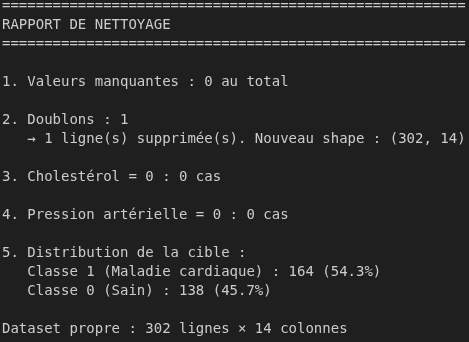
\includegraphics[width=1\textwidth]{./images/nettoyage/nettoyage.png}
			\caption{Rapport de nettoyage}
		\end{figure}

		\begin{tcolorbox}[warnbox, title={Distribution de la variable cible}]
		\begin{itemize}
			\item Classe 0 — Sain : \textbf{138 patients} (45{,}7\,\%)
			\item Classe 1 — Maladie cardiaque : \textbf{164 patients} (54{,}3\,\%)
		\end{itemize}
		Le dataset est pratiquement \textbf{équilibré}, ce qui rend la métrique \metric{Accuracy} fiable et ne nécessite pas de rééchantillonnage (SMOTE).
		\end{tcolorbox}

	\section{Analyse Exploratoire des Données (EDA)}

		\subsection{Distributions univariées}
		
		\paragraph{Distribution de l'âge.} Les patients sont âgés de 29 à 77 ans, avec une médiane autour de 55 ans. Les patients malades sont légèrement plus jeunes en moyenne, ce qui peut sembler contre-intuitif mais s'explique par un biais de sélection de l'échantillon clinique.
		\begin{figure}[H]
			\centering
			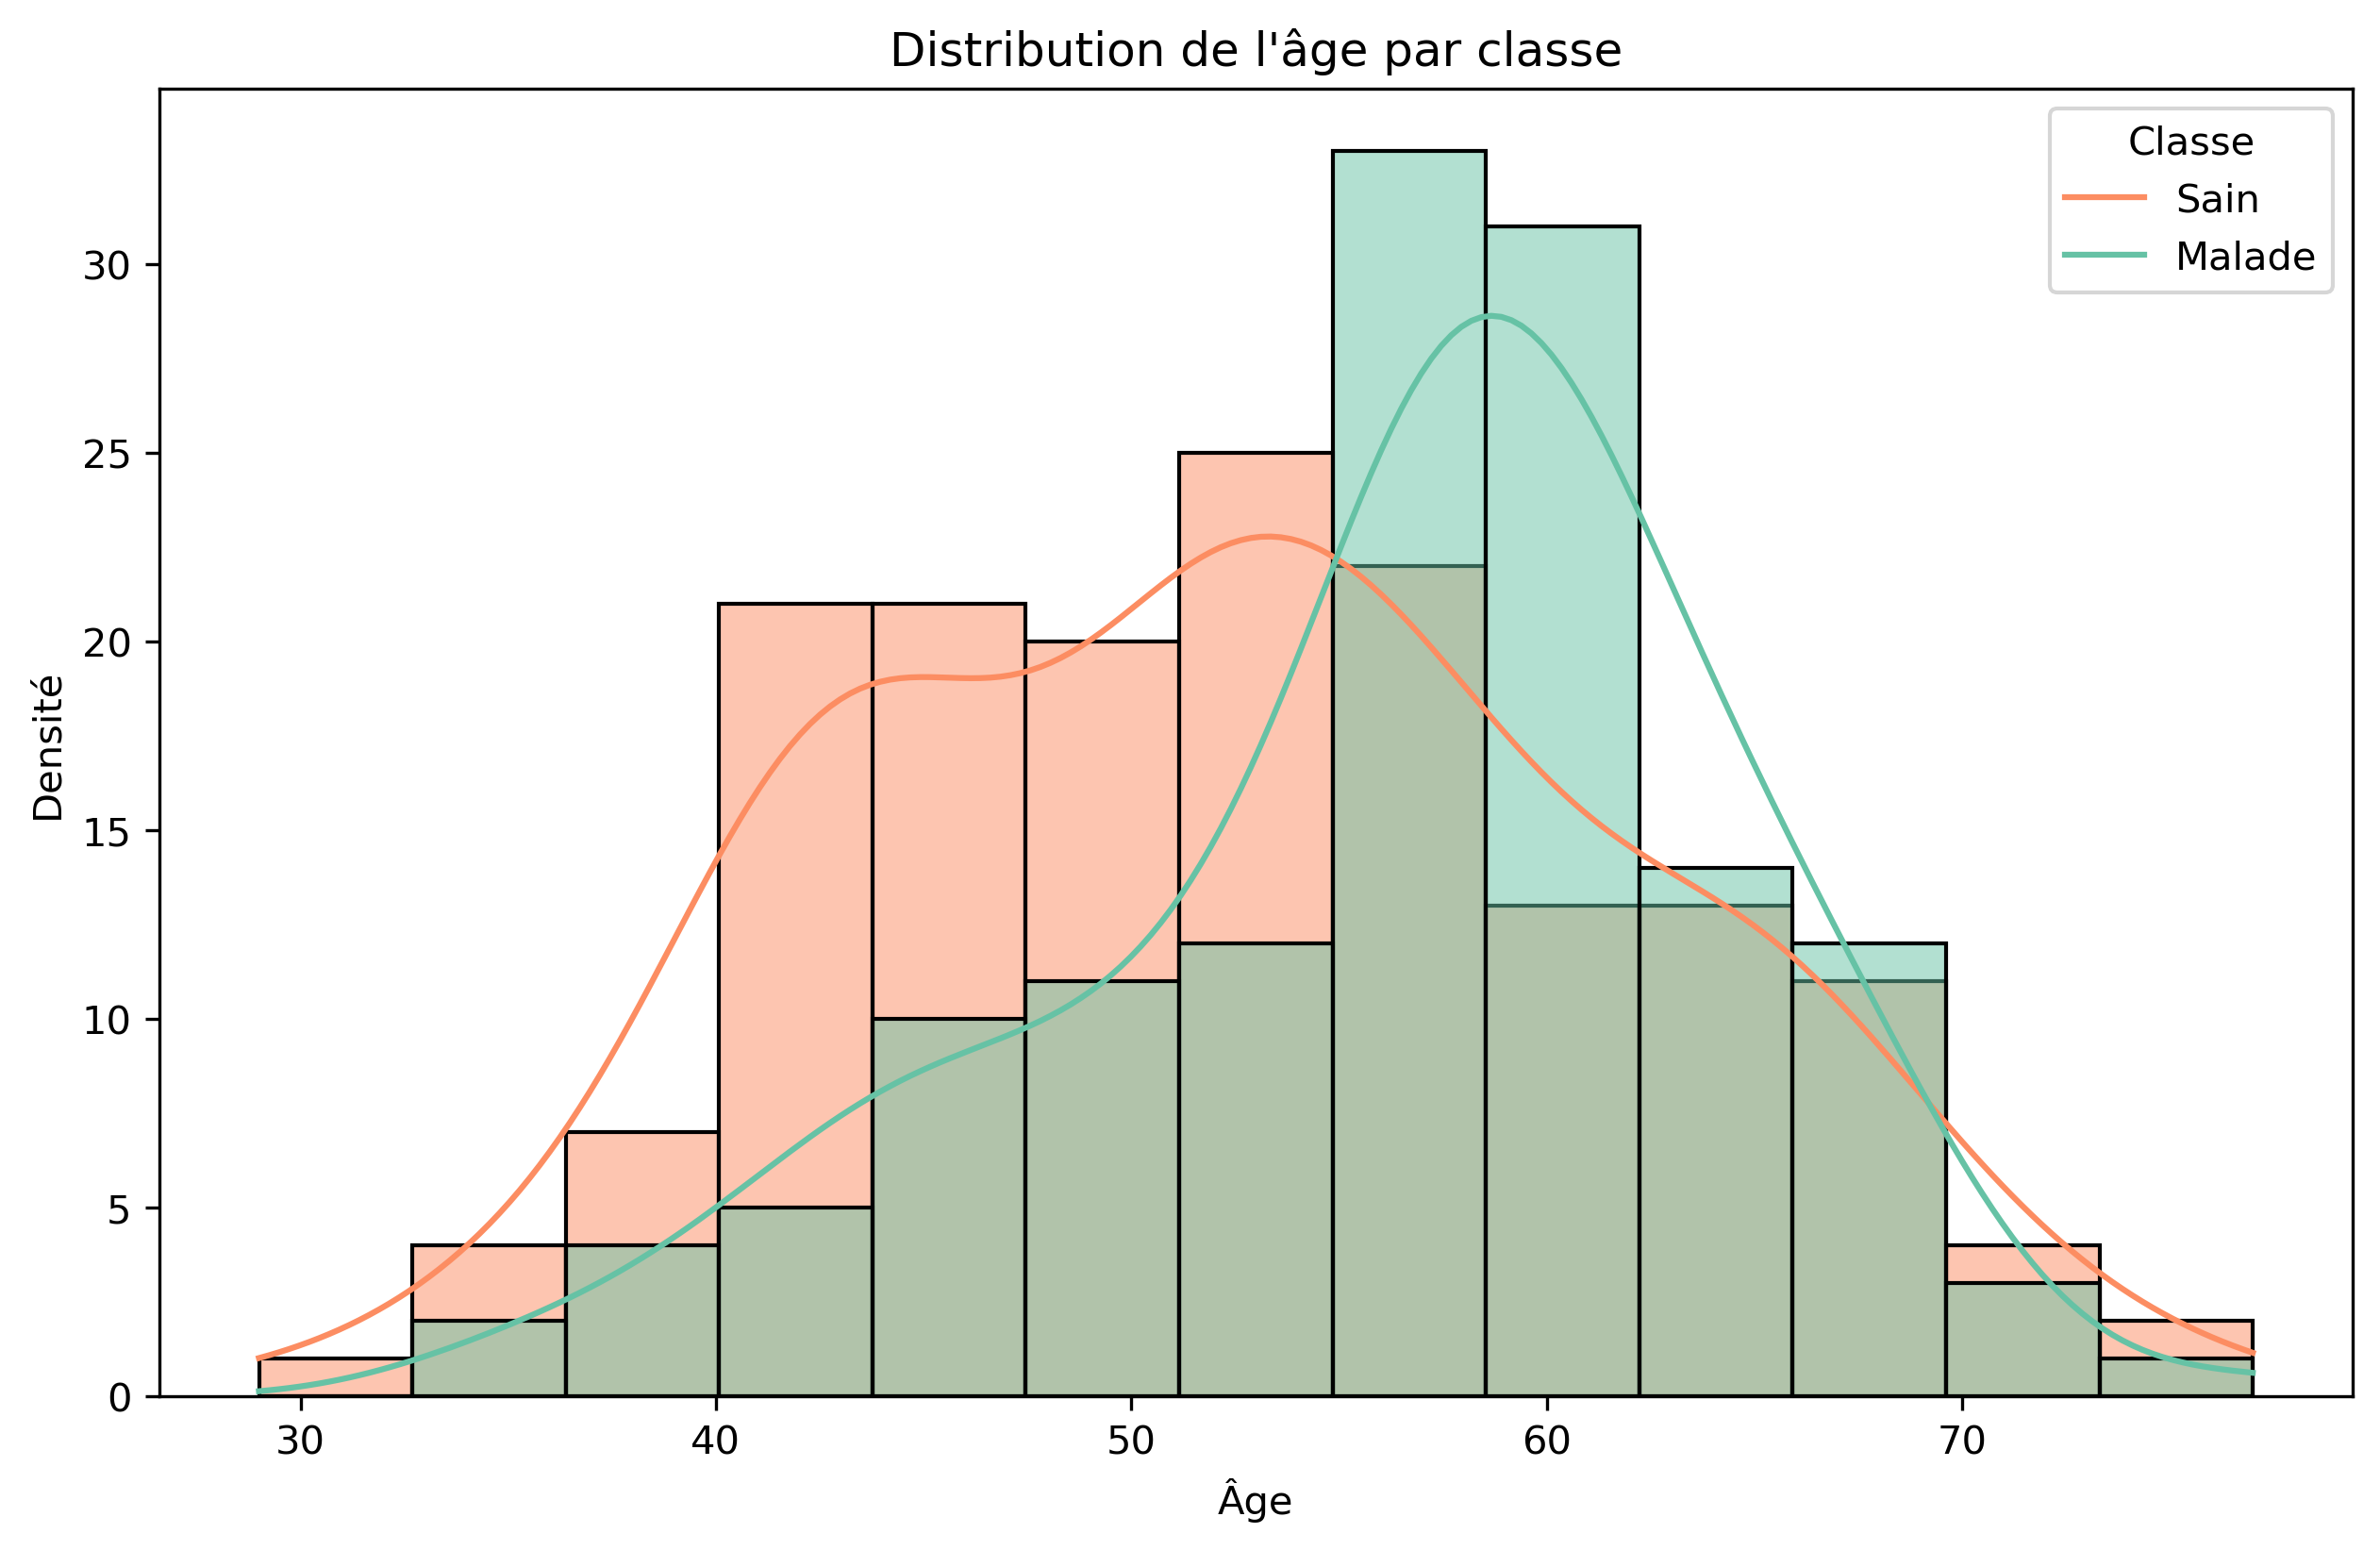
\includegraphics[width=1\textwidth,height=0.6\textwidth]{./images/EDA/age_distribution.png}
			\caption{Distributions des variables continues par classe cible}
		\end{figure}
		\paragraph{Fréquence cardiaque maximale (\feat{thalach}).} Les patients sains présentent une fréquence cardiaque maximale plus élevée. Une \feat{thalach} élevée est généralement signe d'un système cardiovasculaire en meilleure santé.
		\begin{figure}[H]
			\centering
			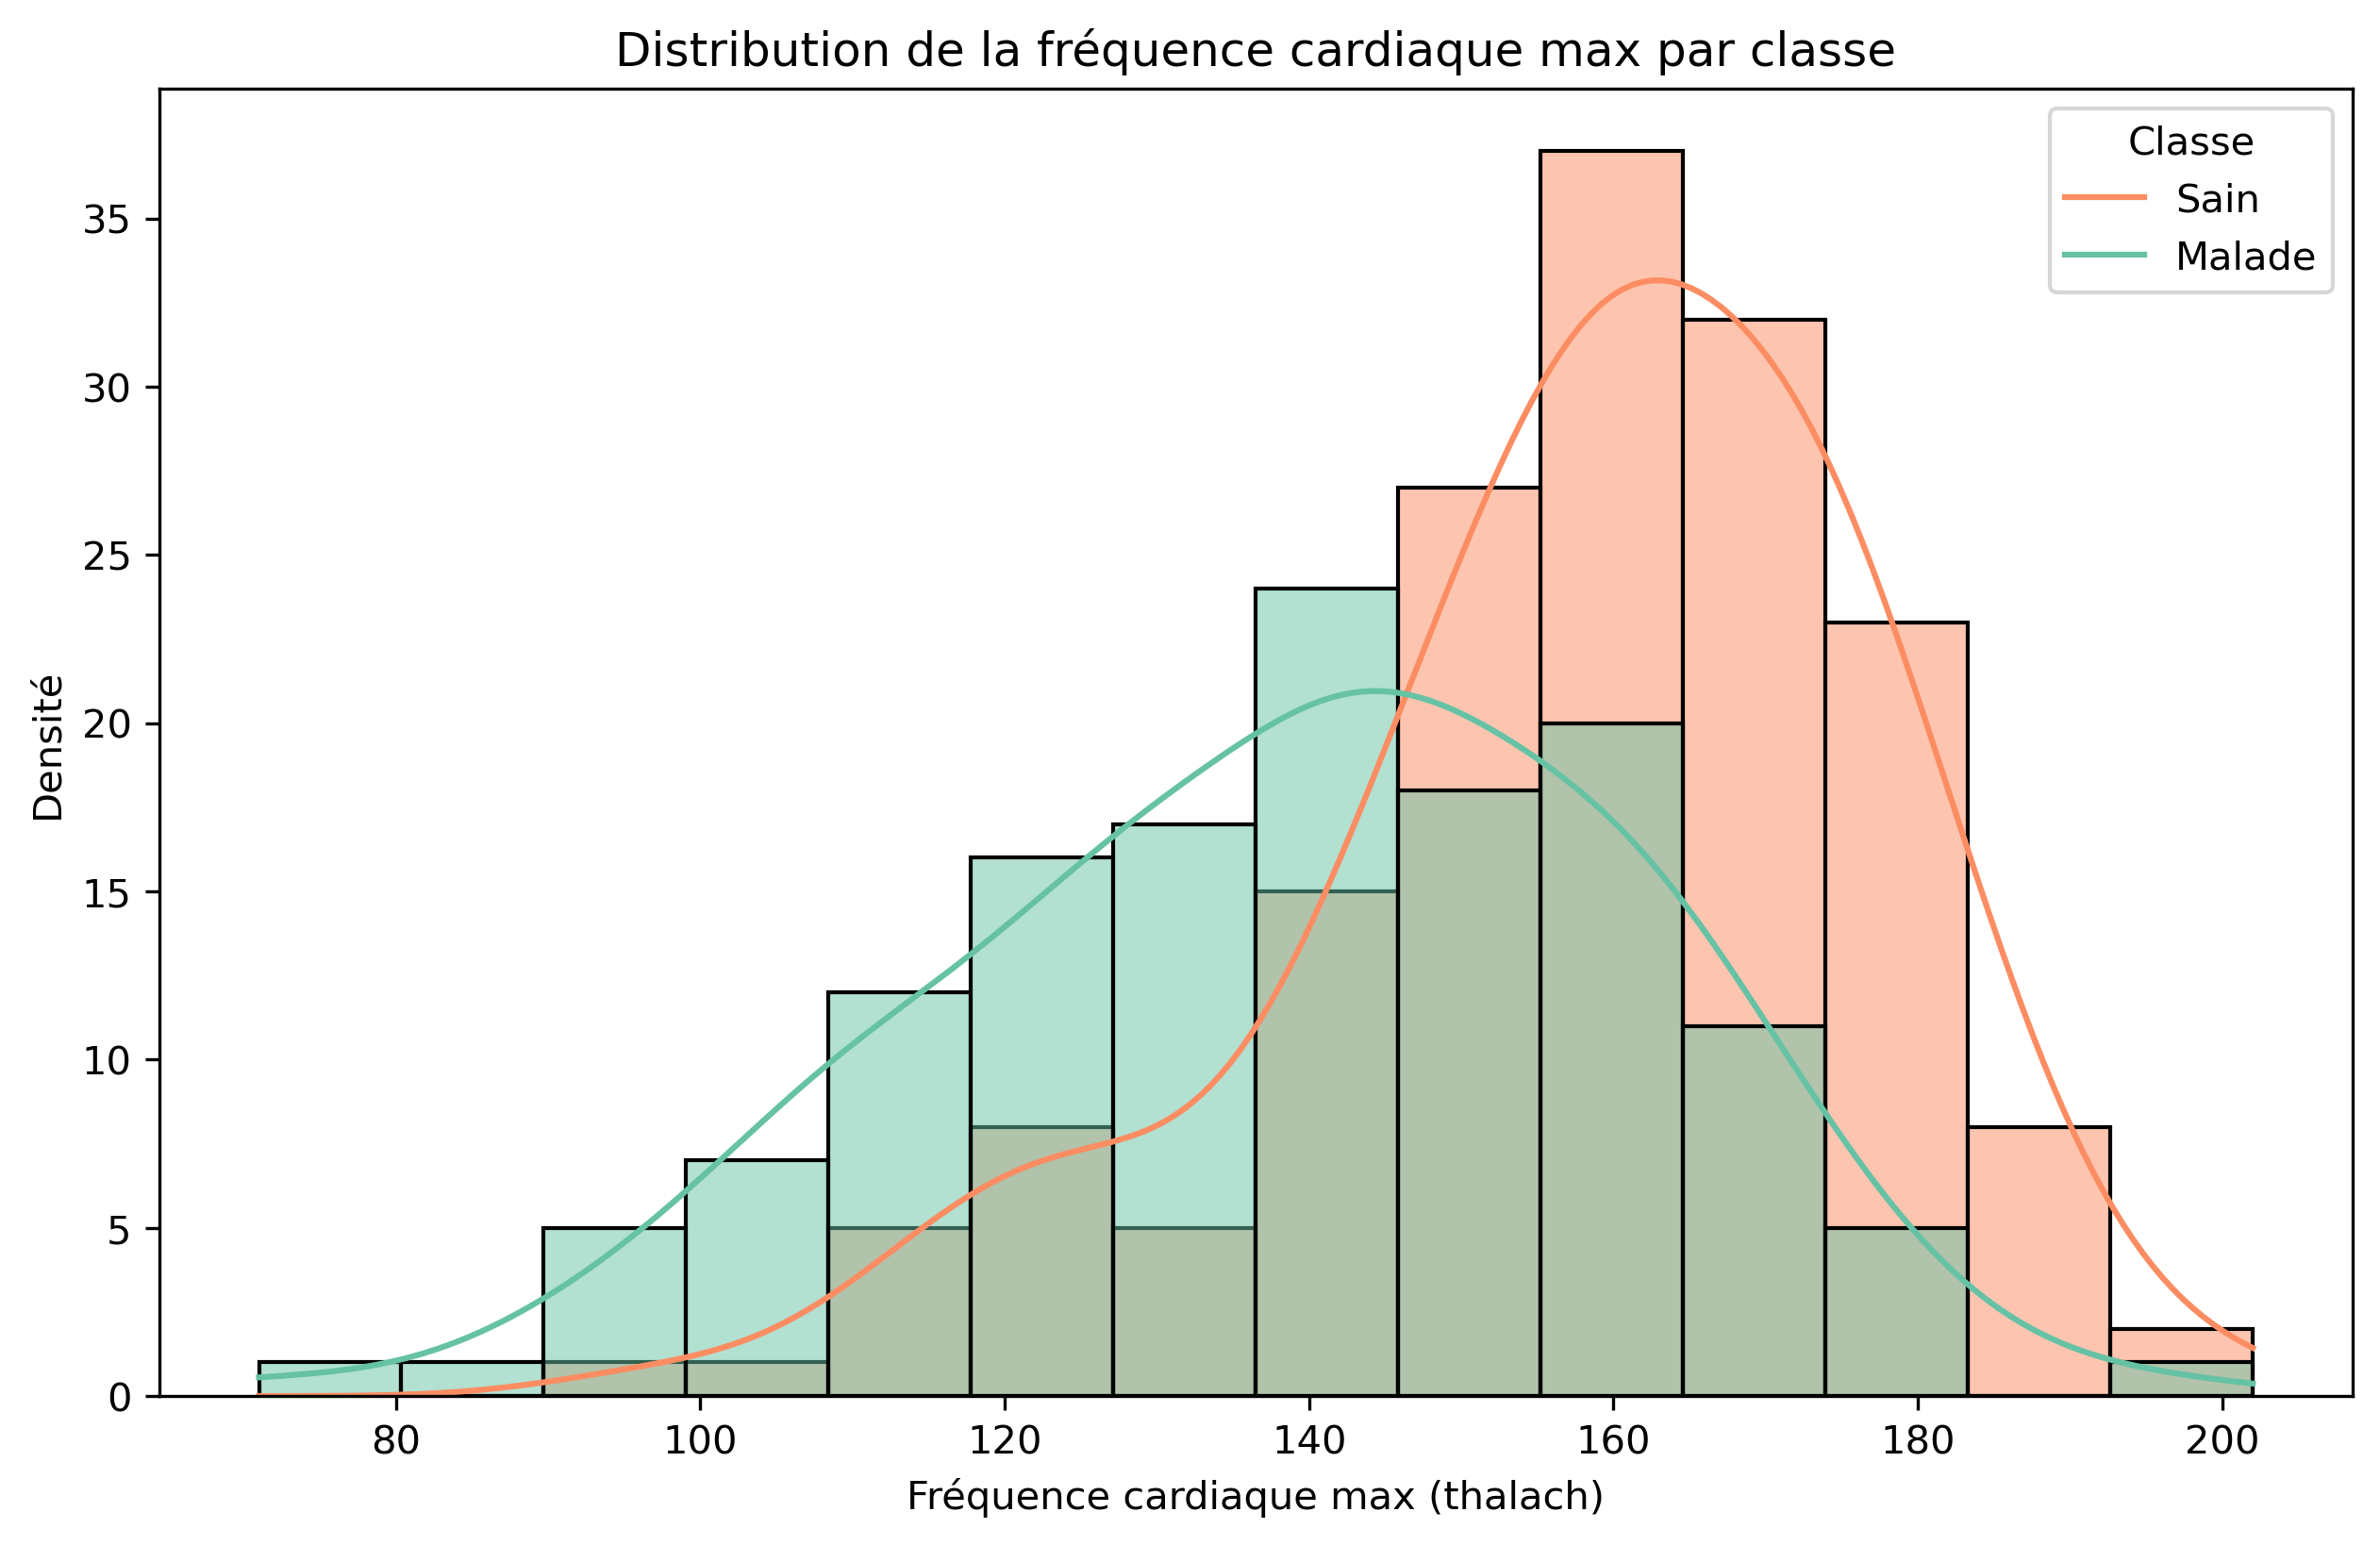
\includegraphics[width=1\textwidth,height=0.6\textwidth]{./images/EDA/thalach_distribution.png}
			\caption{Distribution de la fréquence cardiaque maximale (\feat{thalach}) par classe cible}
			
		\end{figure}
		\paragraph{Dépression du segment ST (\feat{oldpeak}).} Les patients malades affichent un \feat{oldpeak} plus élevé, ce qui est cohérent avec la physiopathologie de l'ischémie myocardique.
		\begin{figure}[H]
			\centering
			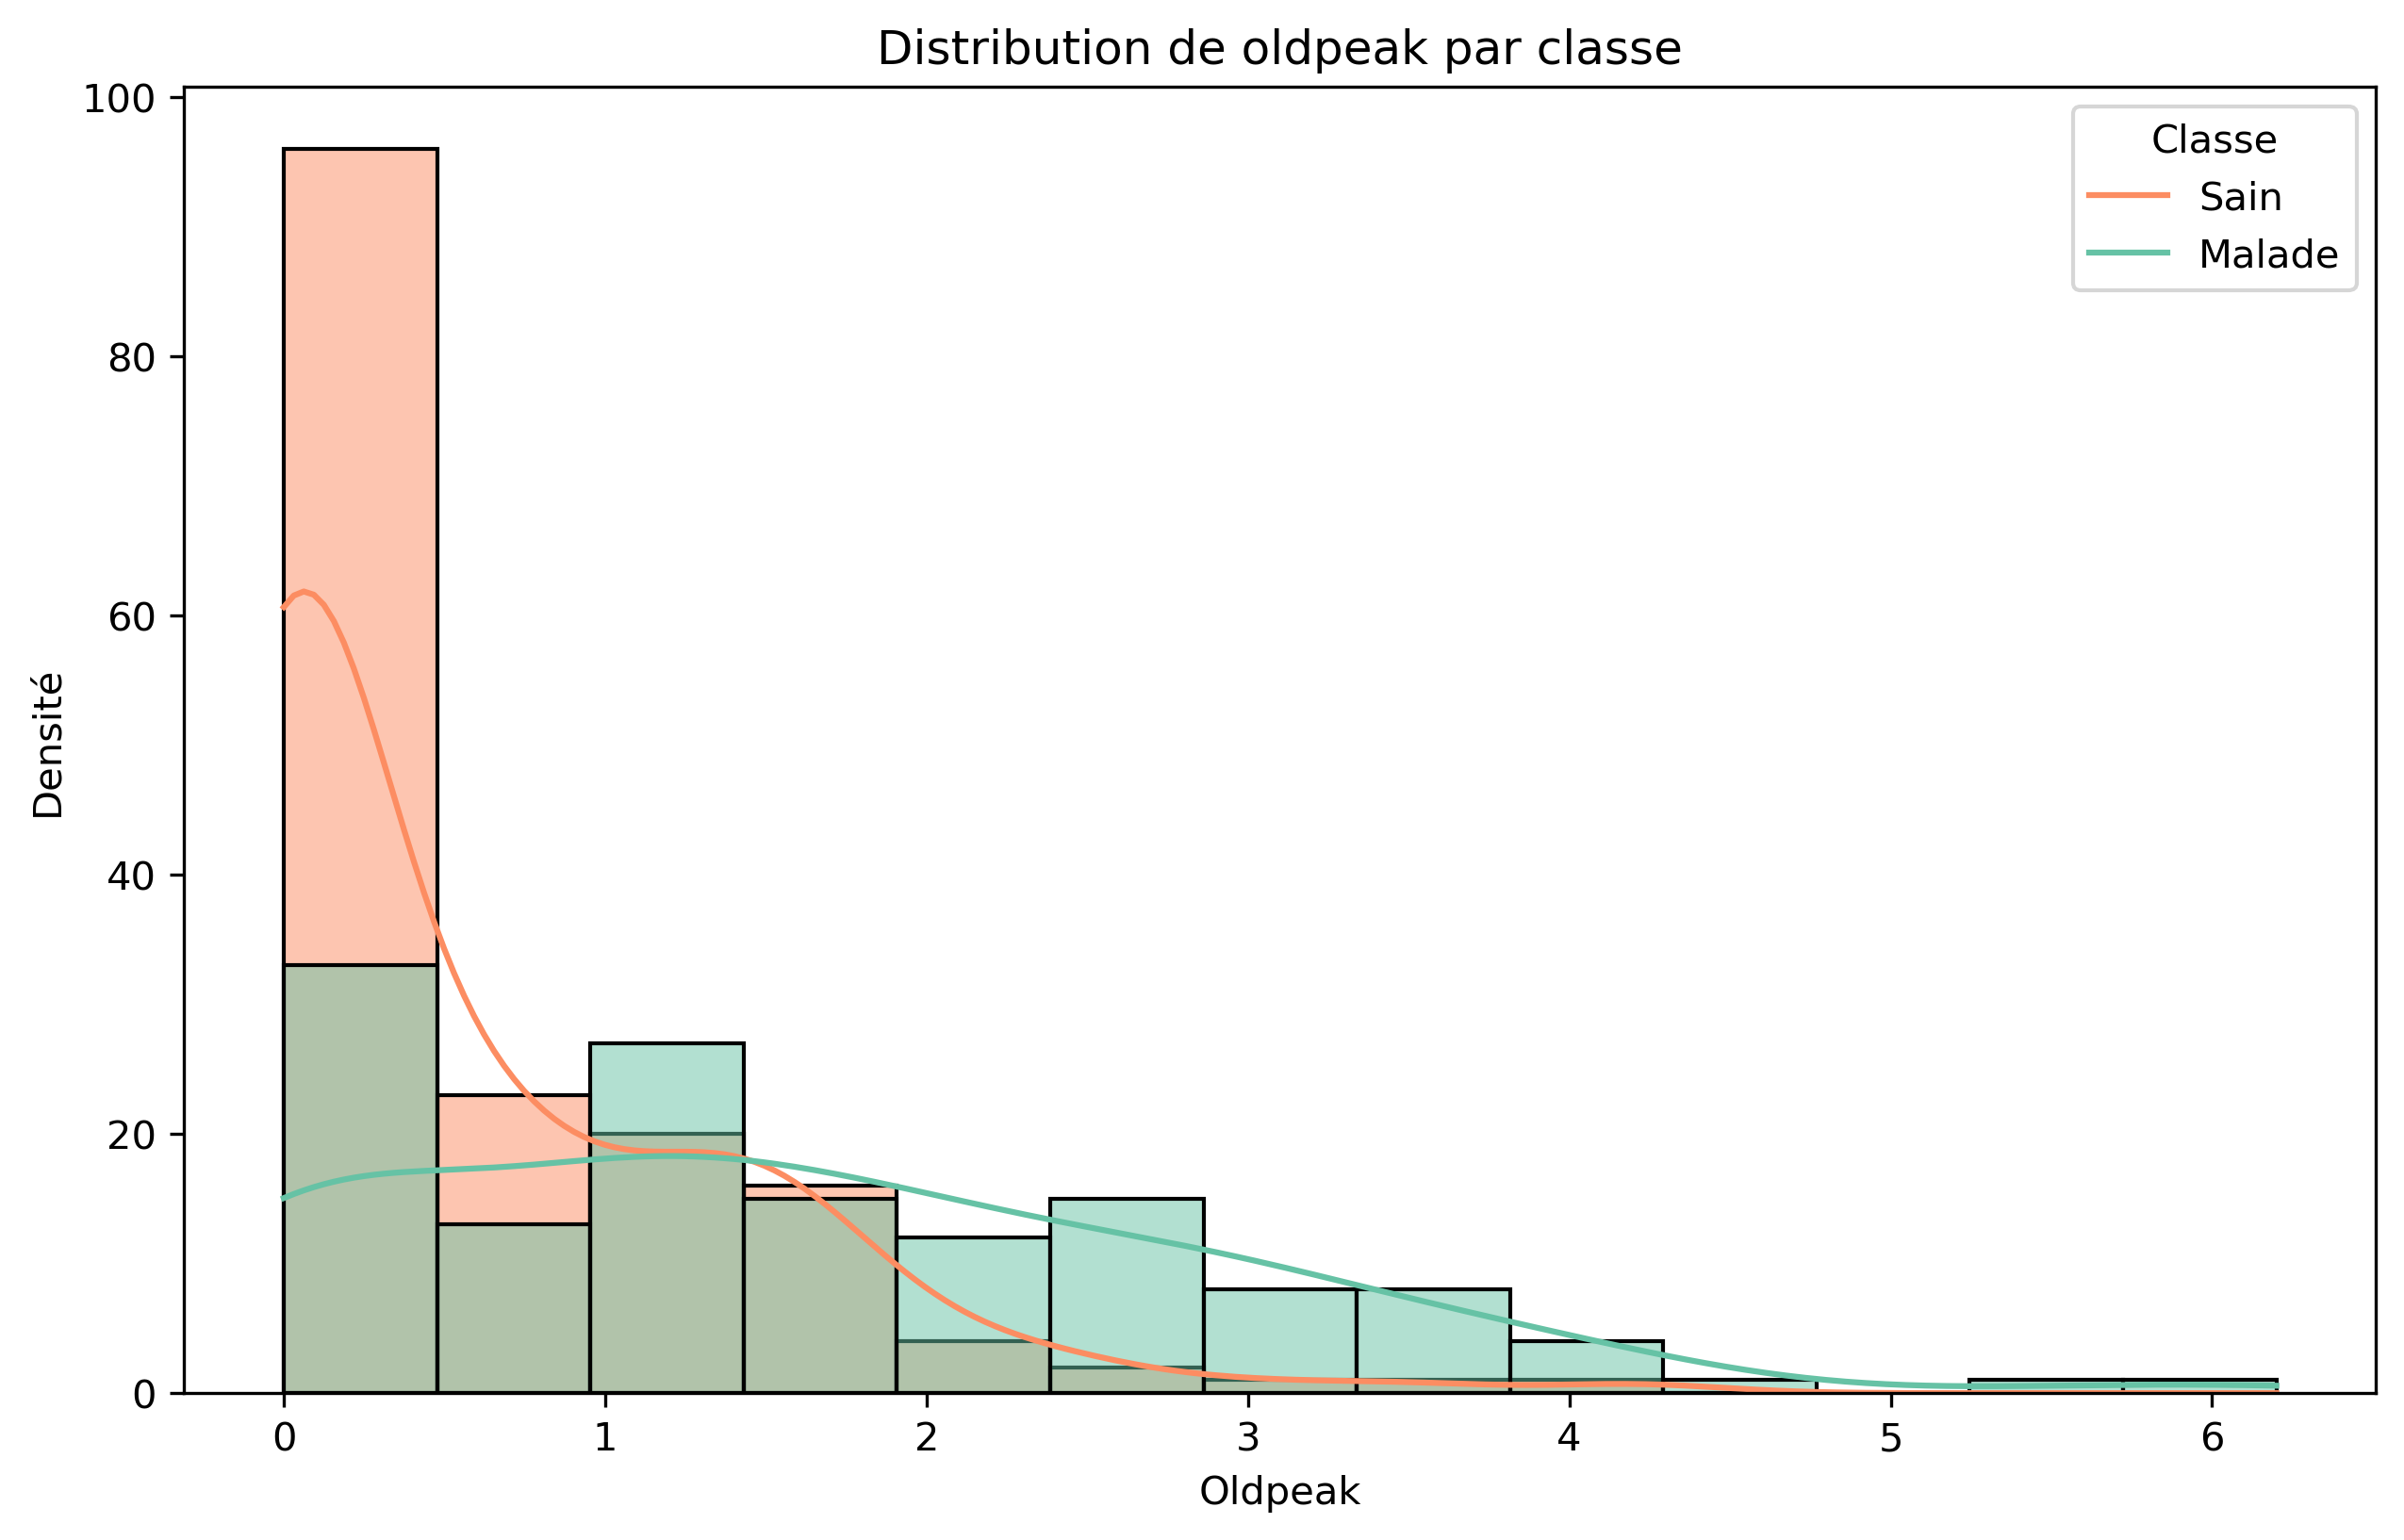
\includegraphics[width=1\textwidth,height=0.6\textwidth]{./images/EDA/oldpeak_distribution.png}
			\caption{Distribution de la dépression du segment ST (\feat{oldpeak}) par classe cible}
		\end{figure}
		\subsection{Variables catégorielles vs cible}

		\begin{figure}[H]
			\centering
			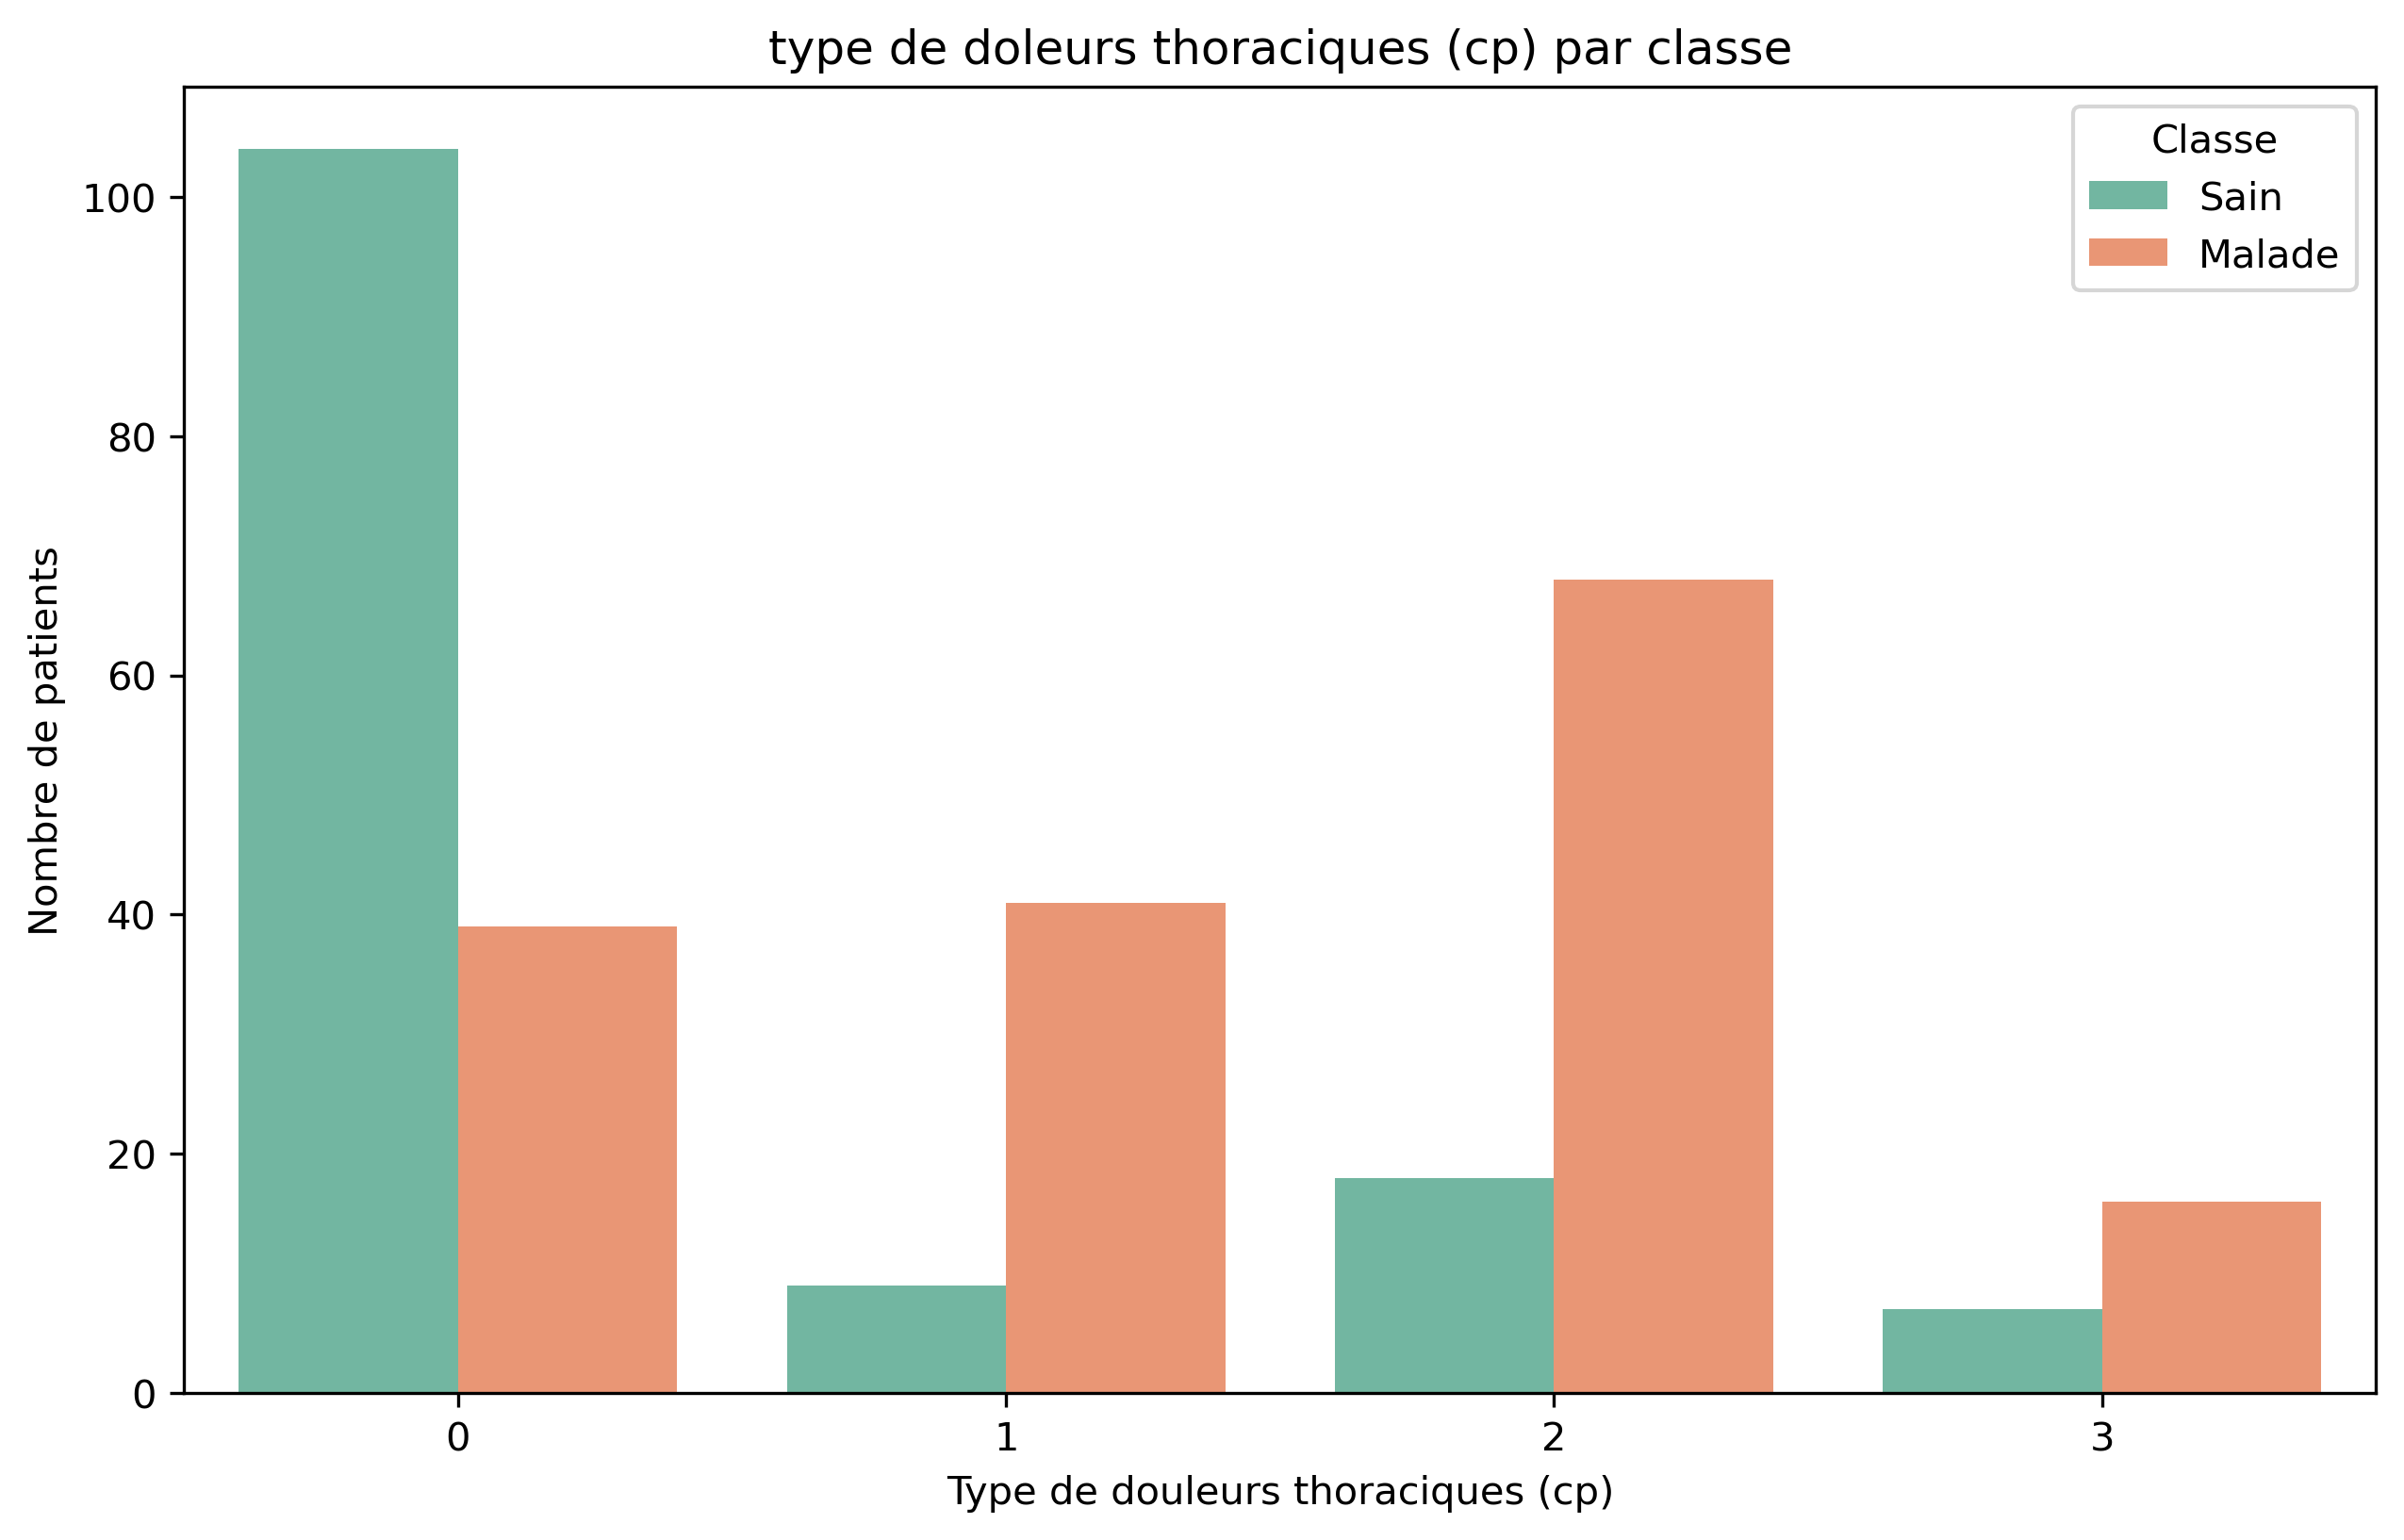
\includegraphics[width=0.48\textwidth]{./images/EDA/cp_target.png}
			\hfill
			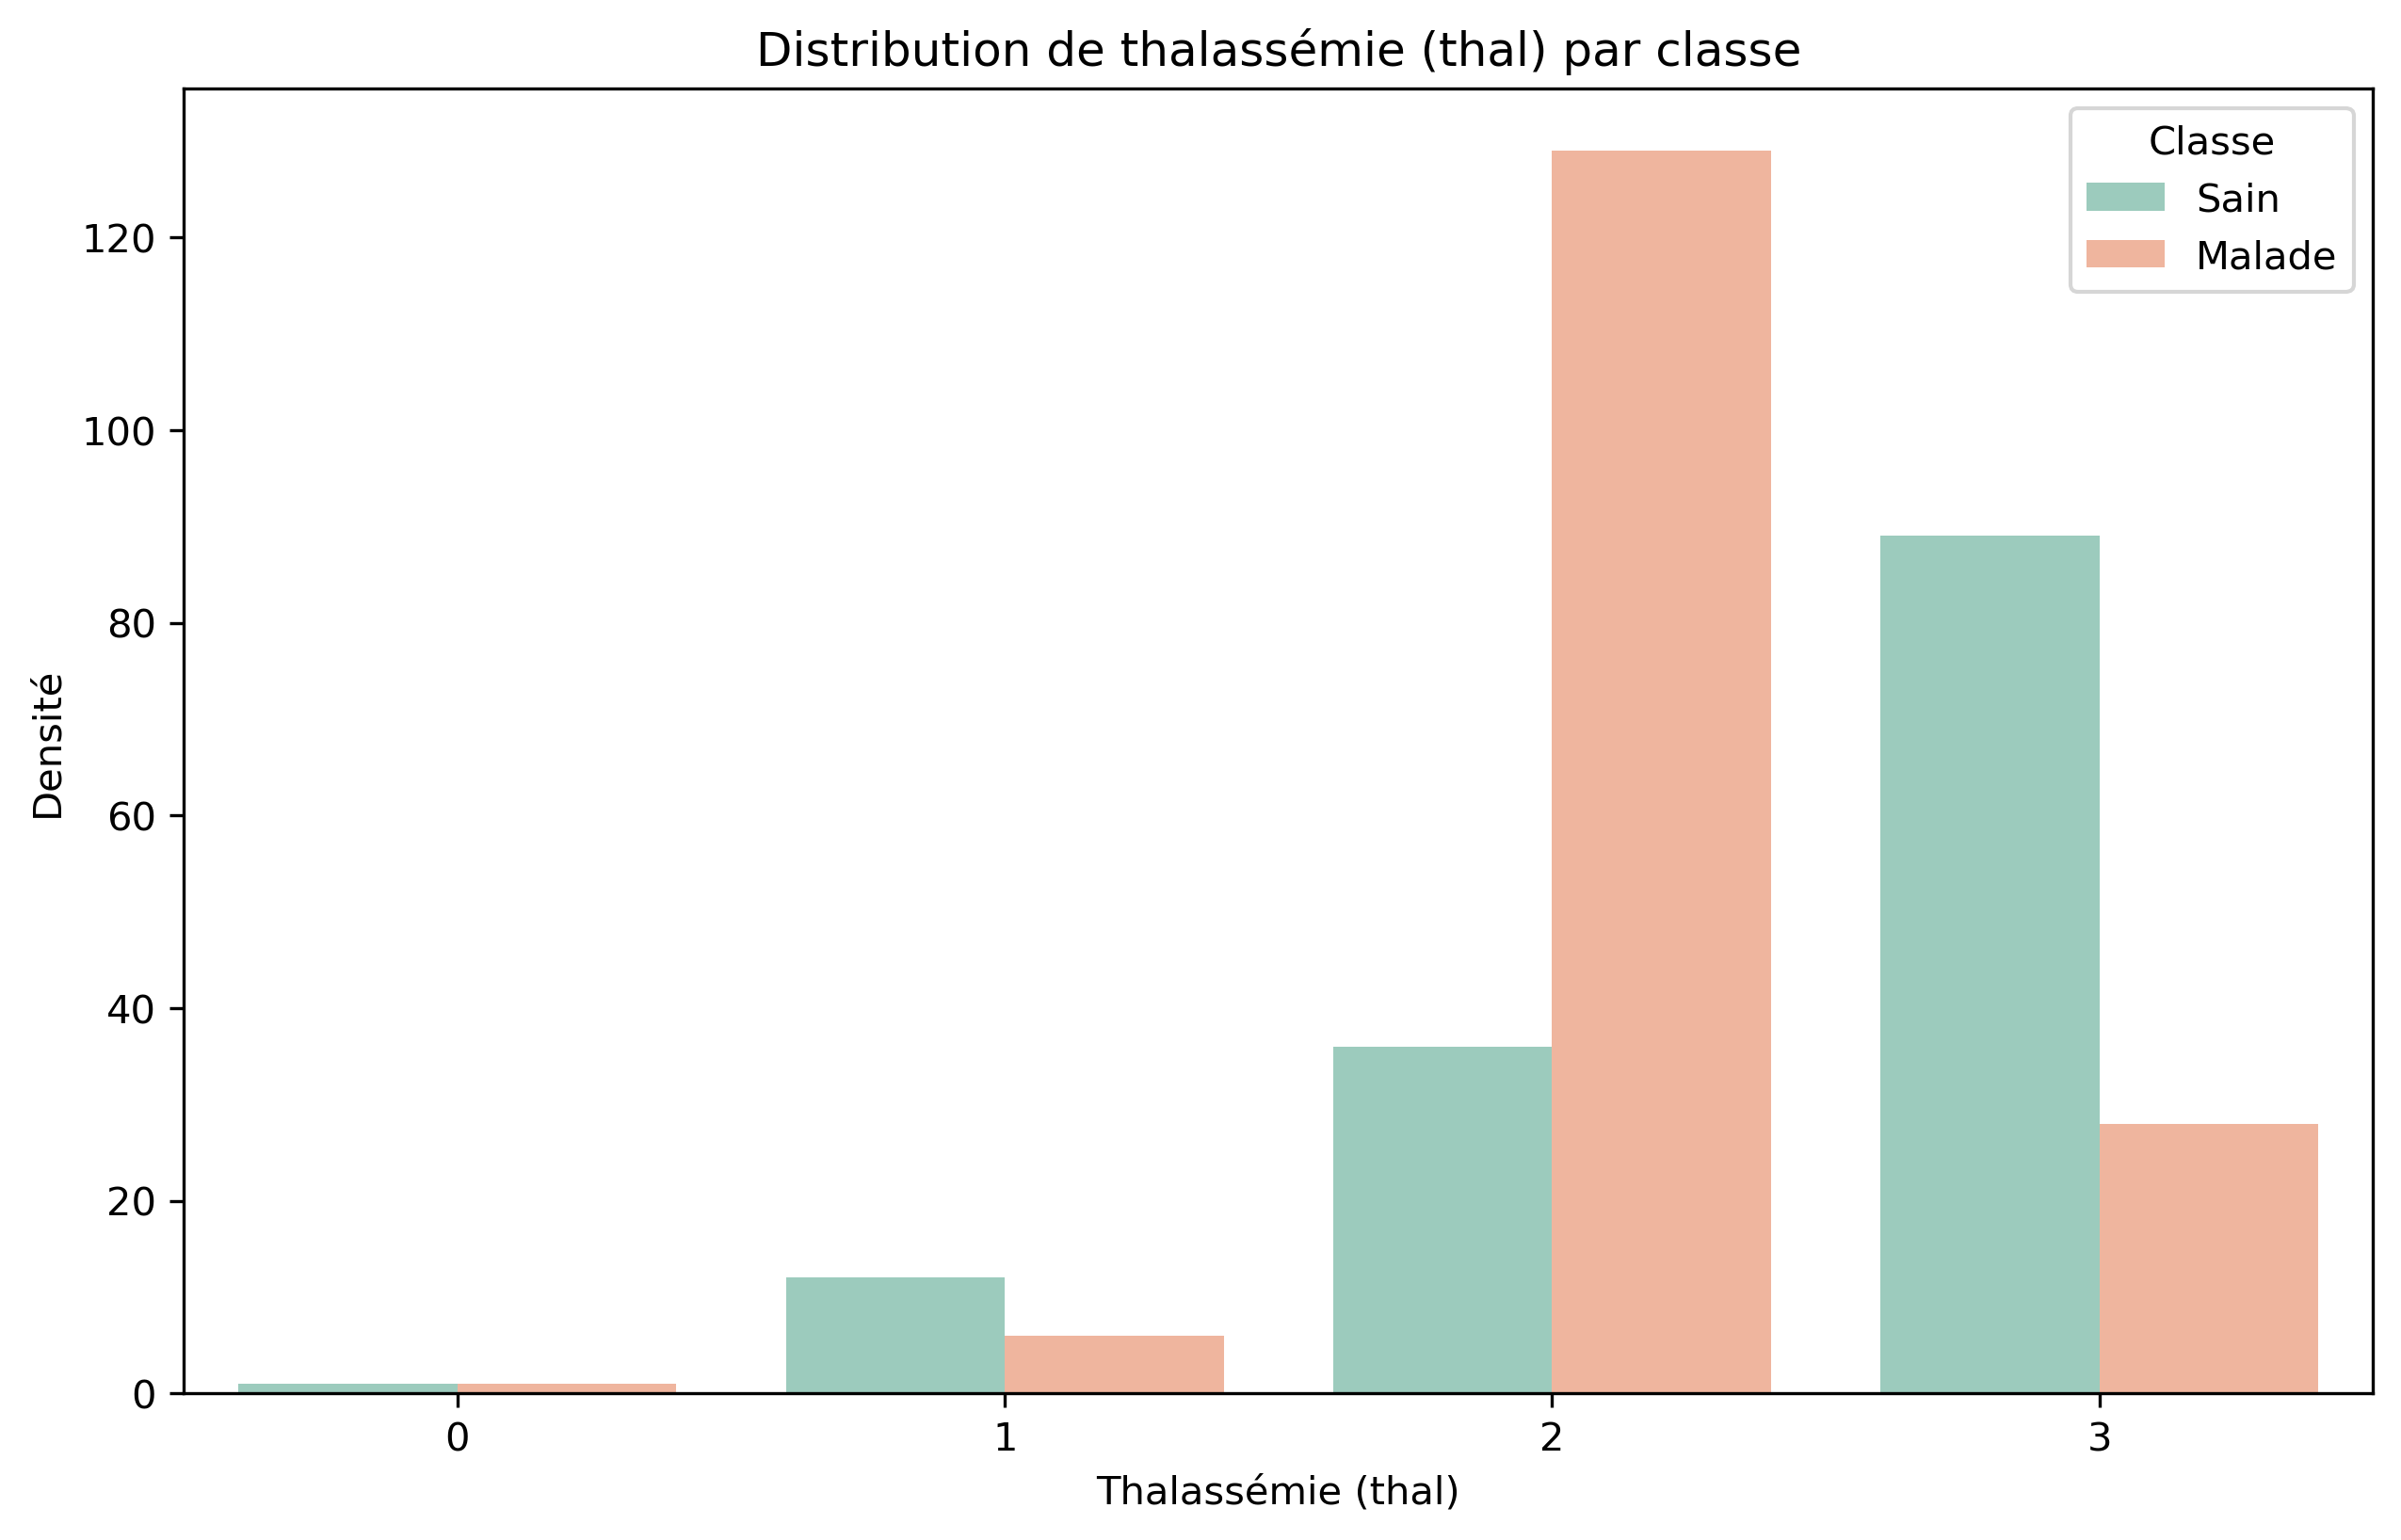
\includegraphics[width=0.48\textwidth]{./images/EDA/thal_distribution.png}
			\linebreak
			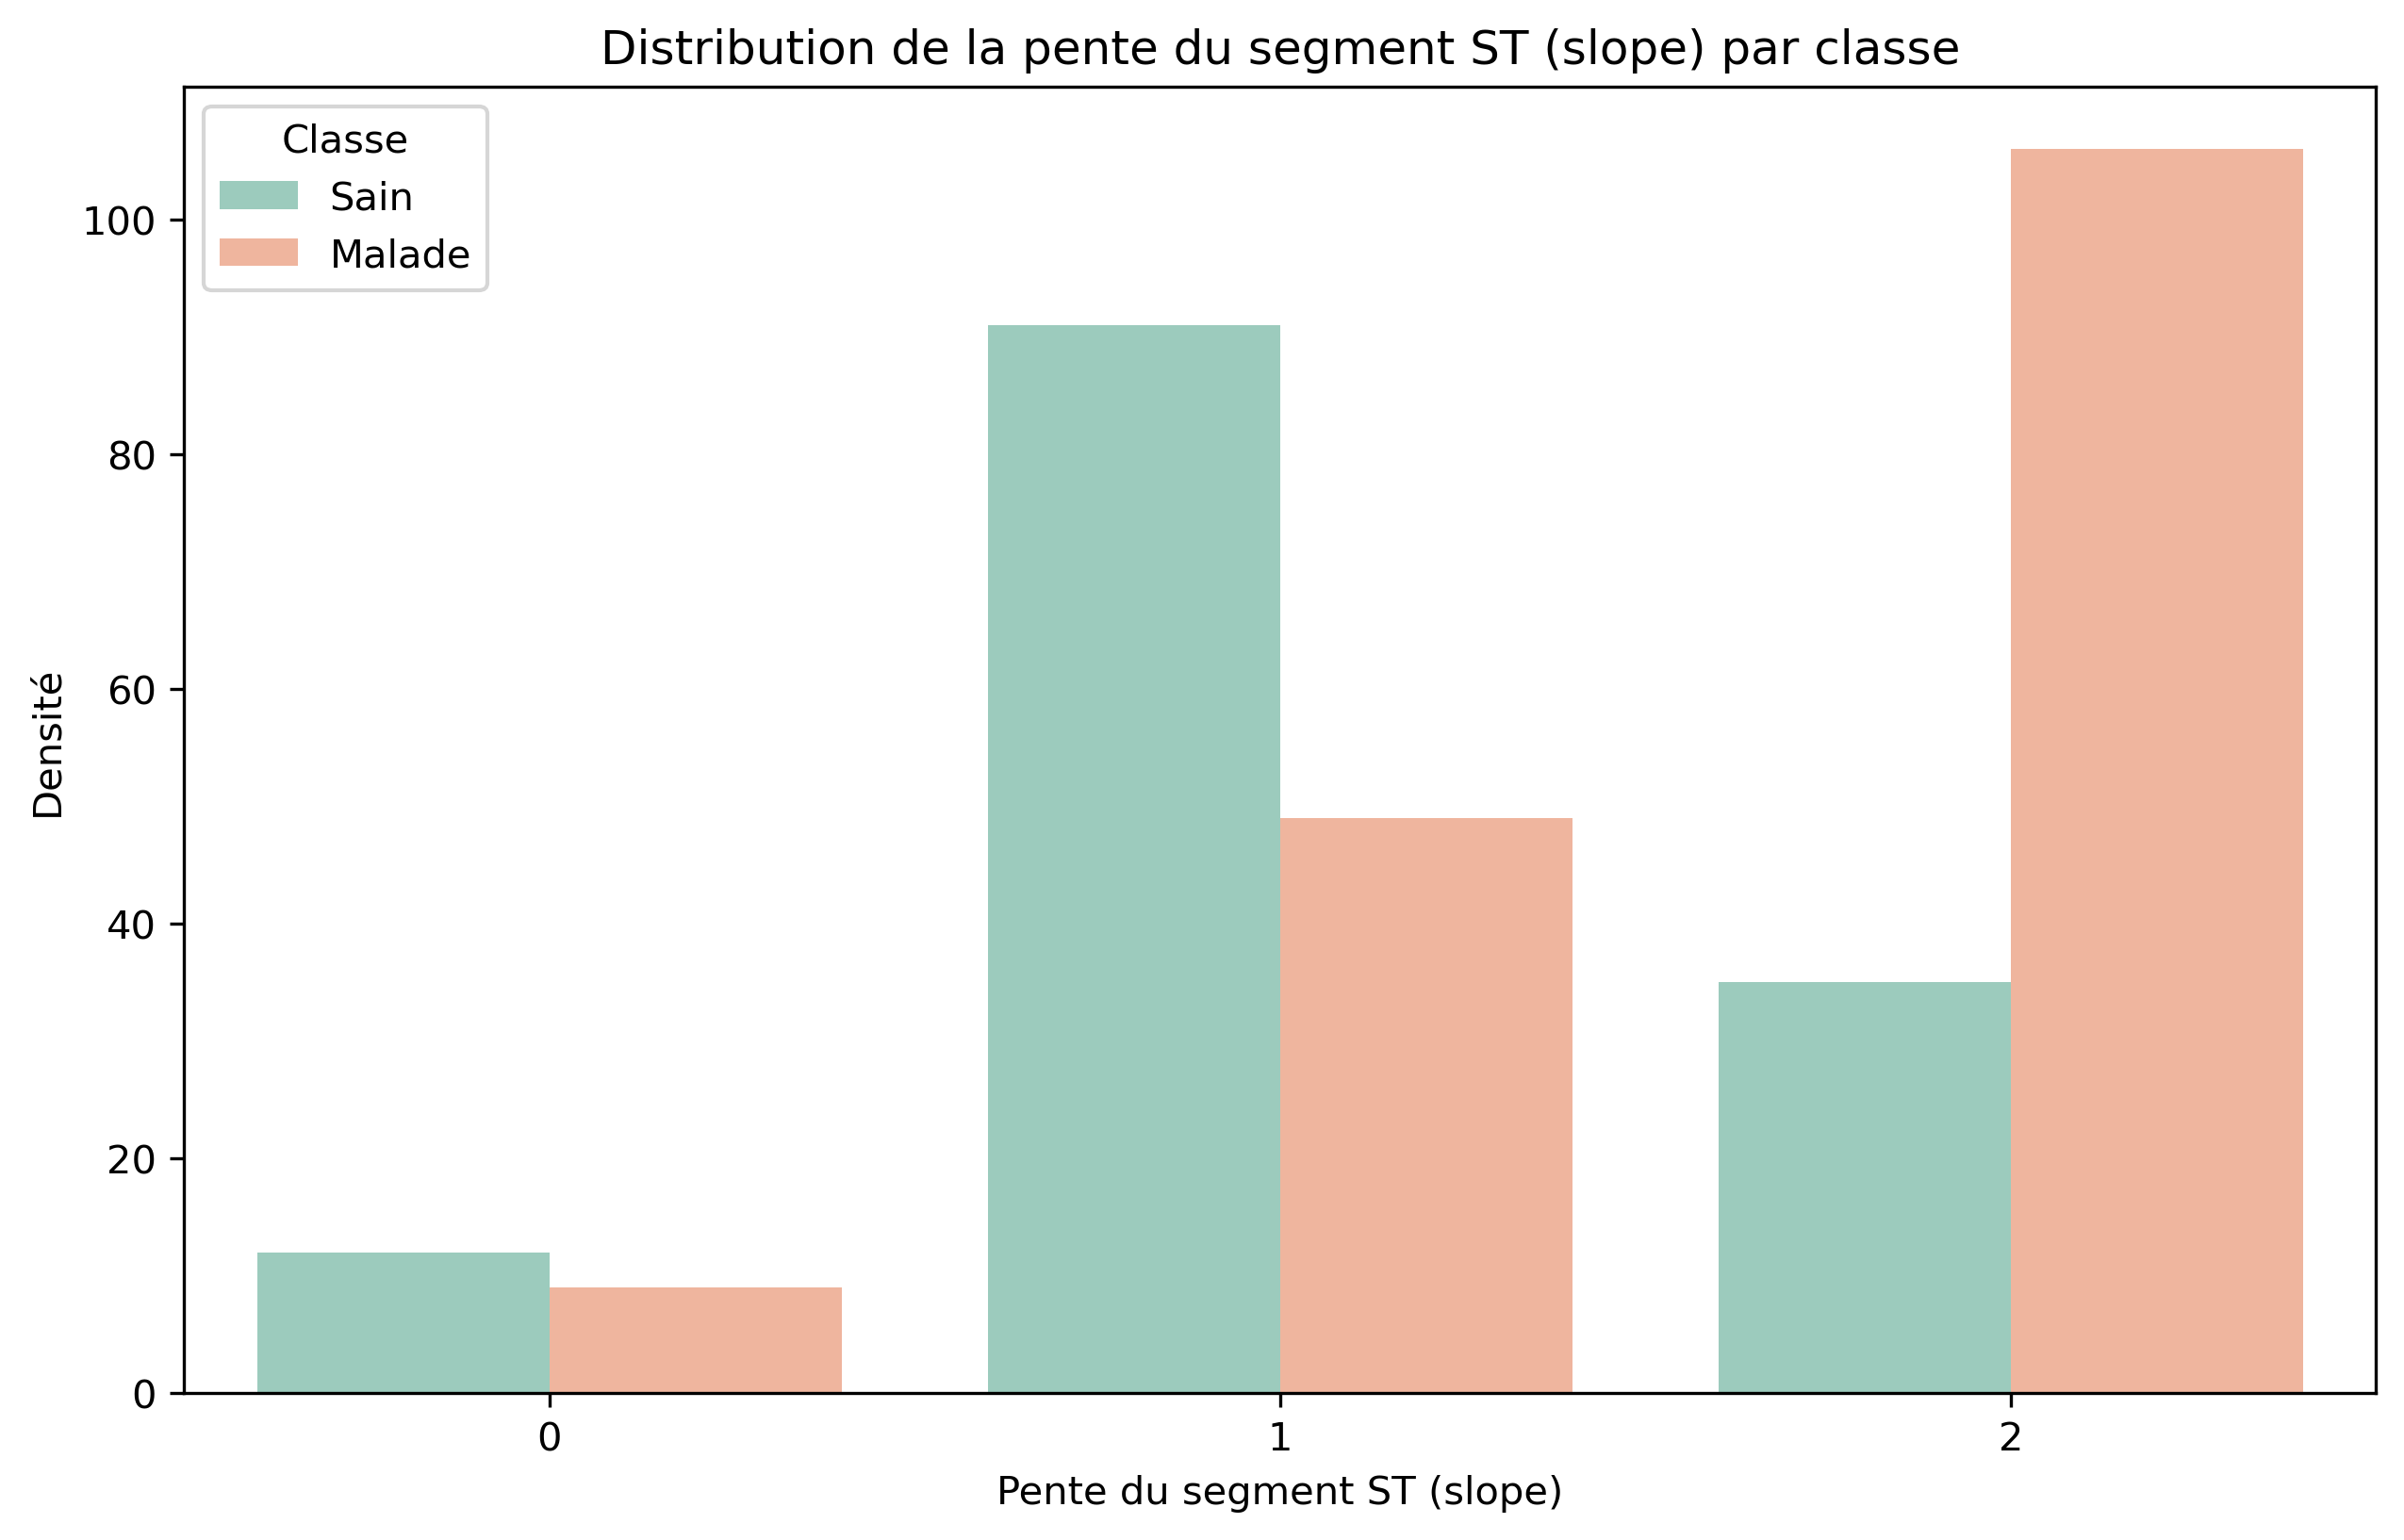
\includegraphics[width=0.48\textwidth]{./images/EDA/slope_distribution.png}
			\caption{Distribution des variables catégorielles par classe cible}
		\end{figure}

		\begin{table}[H]
		\centering
		\caption{Interprétation des variables catégorielles les plus discriminantes}
		\label{tab:cat}
			\begin{tabularx}{\textwidth}{lX}
				\toprule
				\textbf{Variable} & \textbf{Observation} \\
				\midrule
				\feat{cp} (douleur thoracique) & La douleur asymptomatique (type 0) est fortement associée aux patients malades — paradoxe clinique important \\
				\feat{thal} (thalassémie) & Le type 2 (flux normal) est associé à l'absence de maladie ; les types 1 et 3 (défects) au groupe malade \\
				\feat{slope} (pente ST) & Une pente descendante est plus fréquente chez les malades \\
				\feat{ca} (vaisseaux colorés) & Plus le nombre de vaisseaux colorés est élevé, plus le risque de maladie augmente \\
				\bottomrule
			\end{tabularx}
		\end{table}
		\subsection{Matrice de corrélation}

		L'analyse de la matrice de corrélation de Pearson révèle les relations suivantes avec la variable cible \feat{target} :

		\begin{table}[H]
		\centering
		\caption{Corrélations avec la cible (valeur absolue, triées par importance)}
		\label{tab:corr}
		\begin{tabular}{lcc}
			\toprule
			\textbf{Feature} & \textbf{Corrélation} & \textbf{Direction} \\
			\midrule
			\feat{thal}     & $-0{,}34$ & Négatif \\
			\feat{cp}       & $+0{,}43$ & Positif \\
			\feat{ca}       & $-0{,}41$ & Négatif \\
			\feat{thalach}  & $+0{,}42$ & Positif \\
			\feat{oldpeak}  & $-0{,}43$ & Négatif \\
			\feat{exang}    & $-0{,}44$ & Négatif \\
			\feat{slope}    & $+0{,}34$ & Positif \\
			\feat{sex}      & $-0{,}28$ & Négatif \\
			\feat{age}      & $-0{,}23$ & Négatif \\
			\bottomrule
		\end{tabular}
		\end{table}

		\begin{figure}[H]
			\centering
			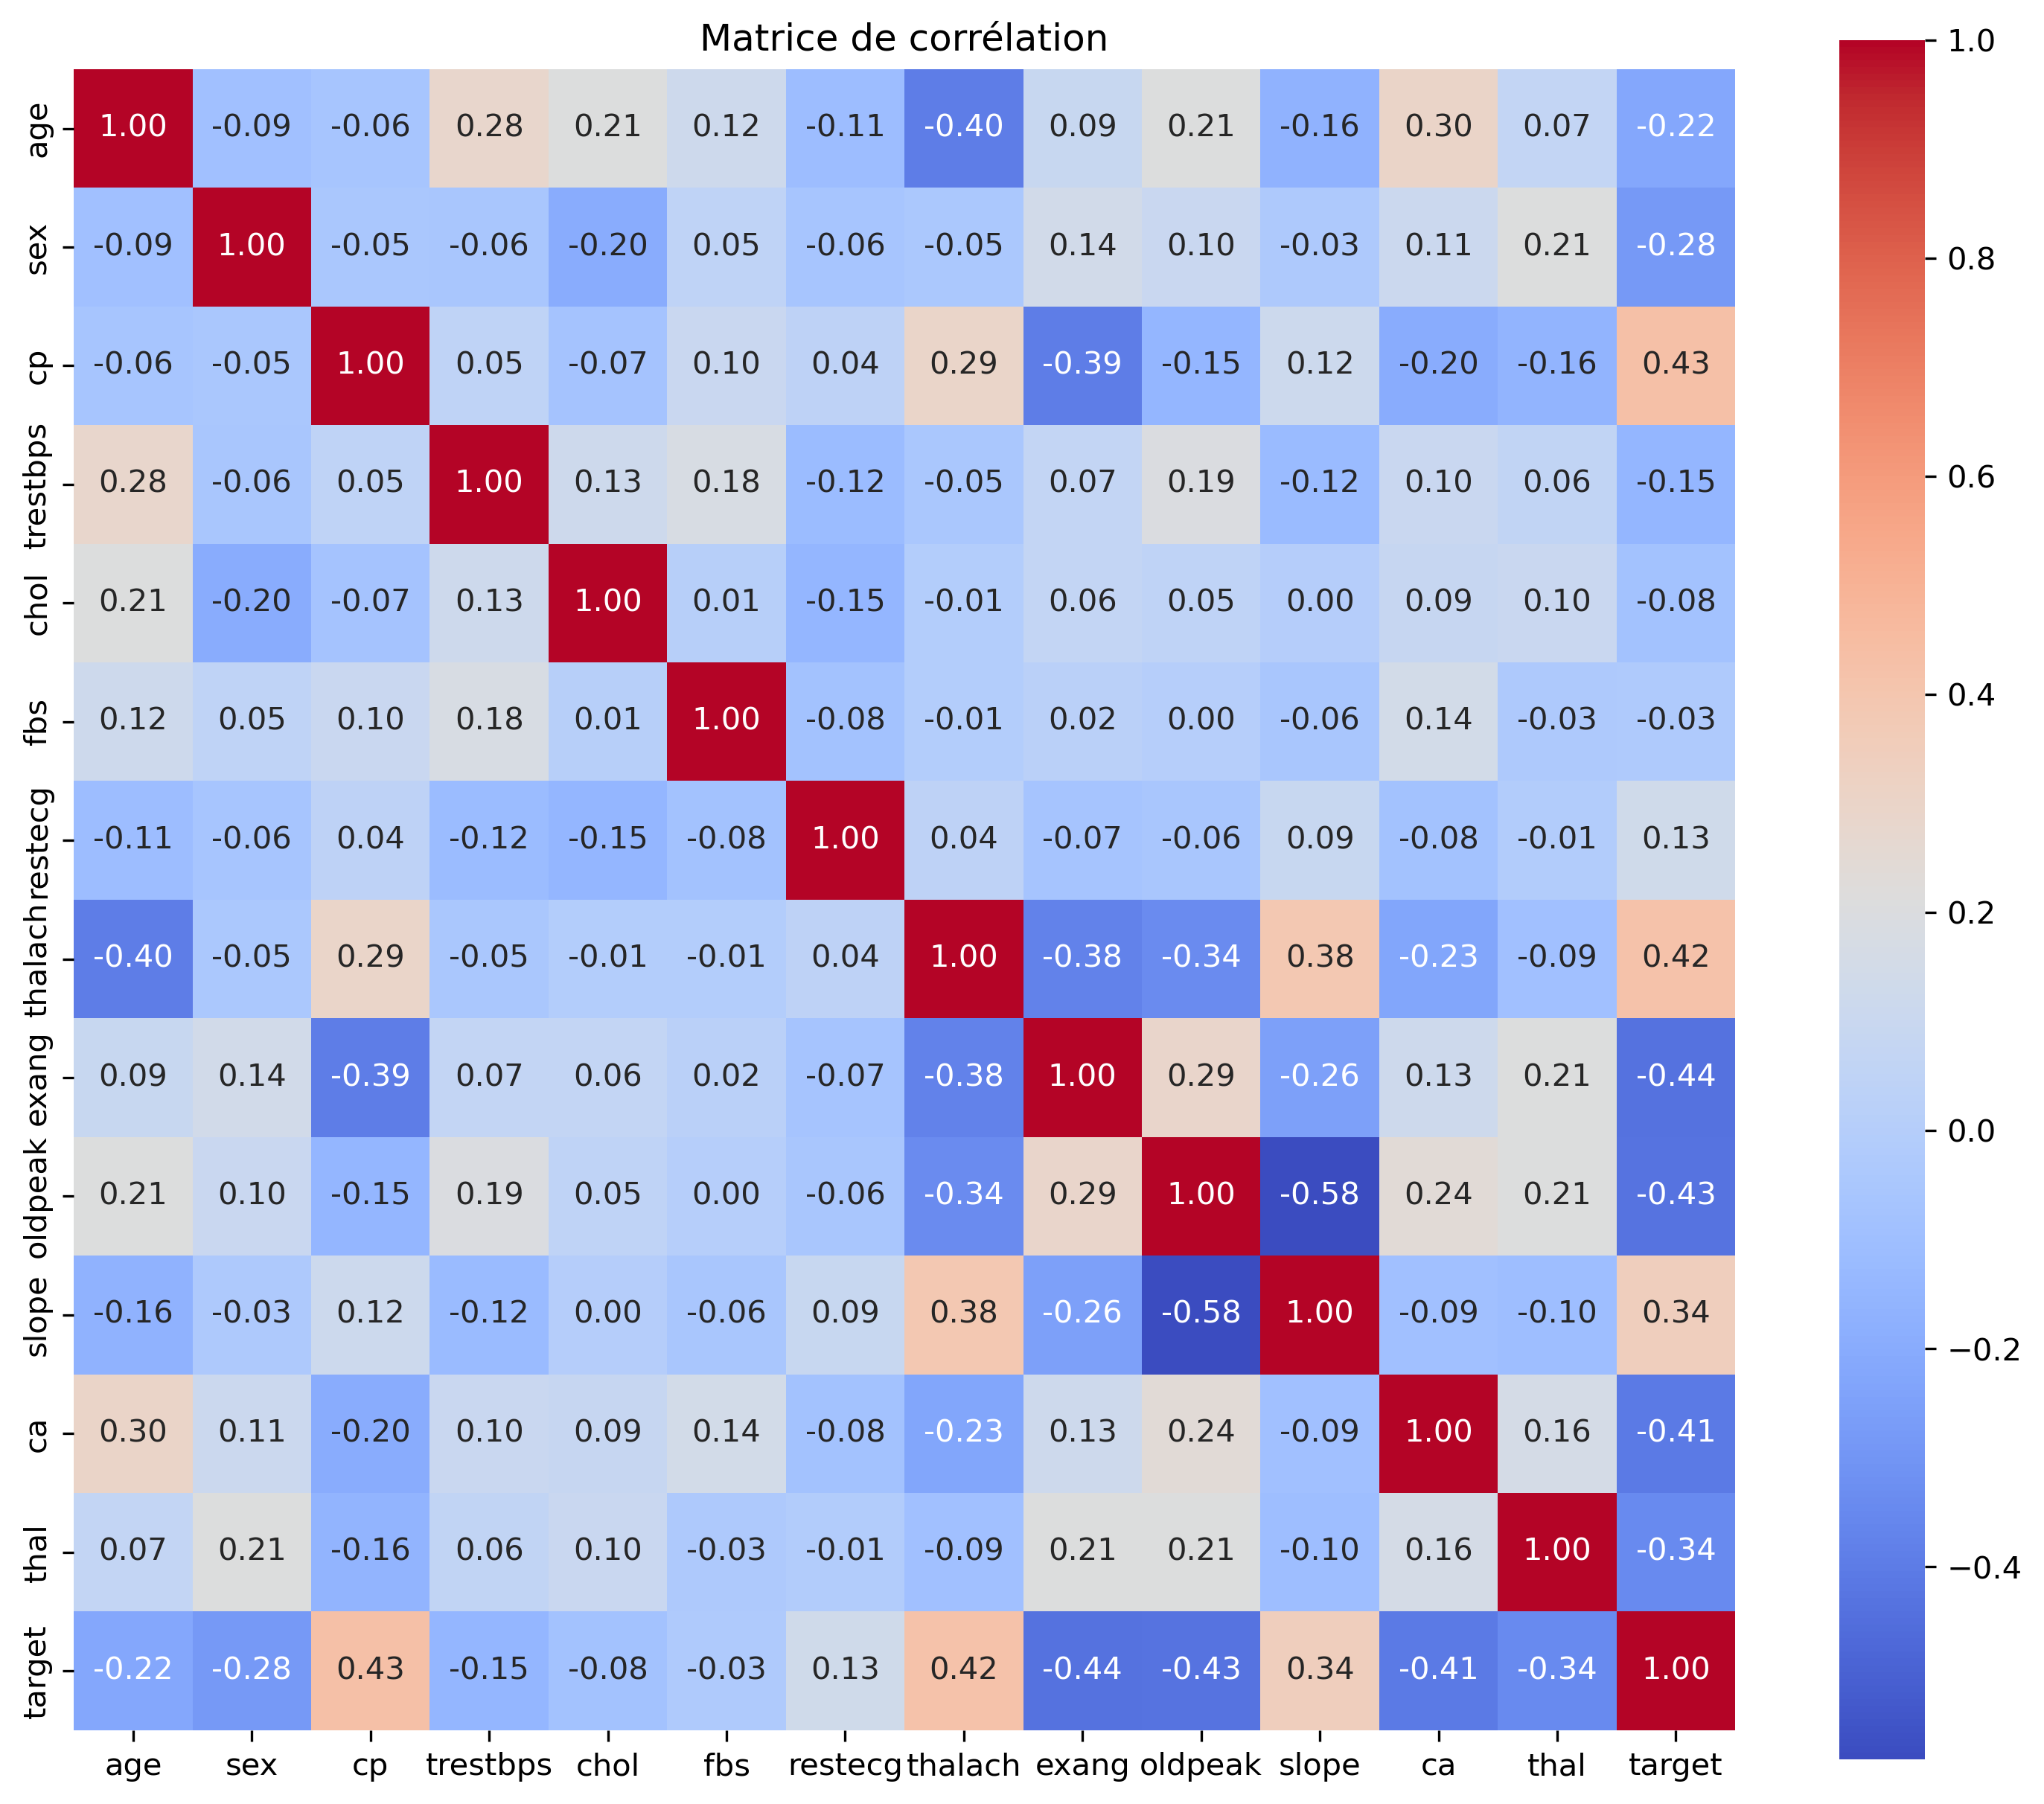
\includegraphics[width=0.8\textwidth,height=0.6\textwidth]{./images/EDA/correlation_matrix.png}
			\caption{Matrice de corrélation de Pearson entre les variables continues et la cible}
		\end{figure}

		\textbf{Observations clés :}
		\begin{itemize}
		\item La corrélation maximale est modérée ($\leq 0{,}43$) : aucune variable n'est à elle seule suffisante pour le diagnostic.
		\item La quasi-absence de corrélation de \feat{fbs} et \feat{restecg} avec la cible suggère leur faible pouvoir prédictif individuel.
		\item Les intercorrélations entre variables explicatives restent raisonnables, limitant le risque de multicolinéarité pour la Régression Logistique.
		\end{itemize}
		\subsection{Analyse par sexe}

		Une disparité notable est observée : les \textbf{femmes} présentent un taux de maladie cardiaque plus élevé dans cet échantillon que les hommes. Ce résultat, contre-intuitif par rapport aux statistiques épidémiologiques générales, reflète le biais de sélection propre à ce dataset clinique.
		\begin{figure}[H]
			\centering
			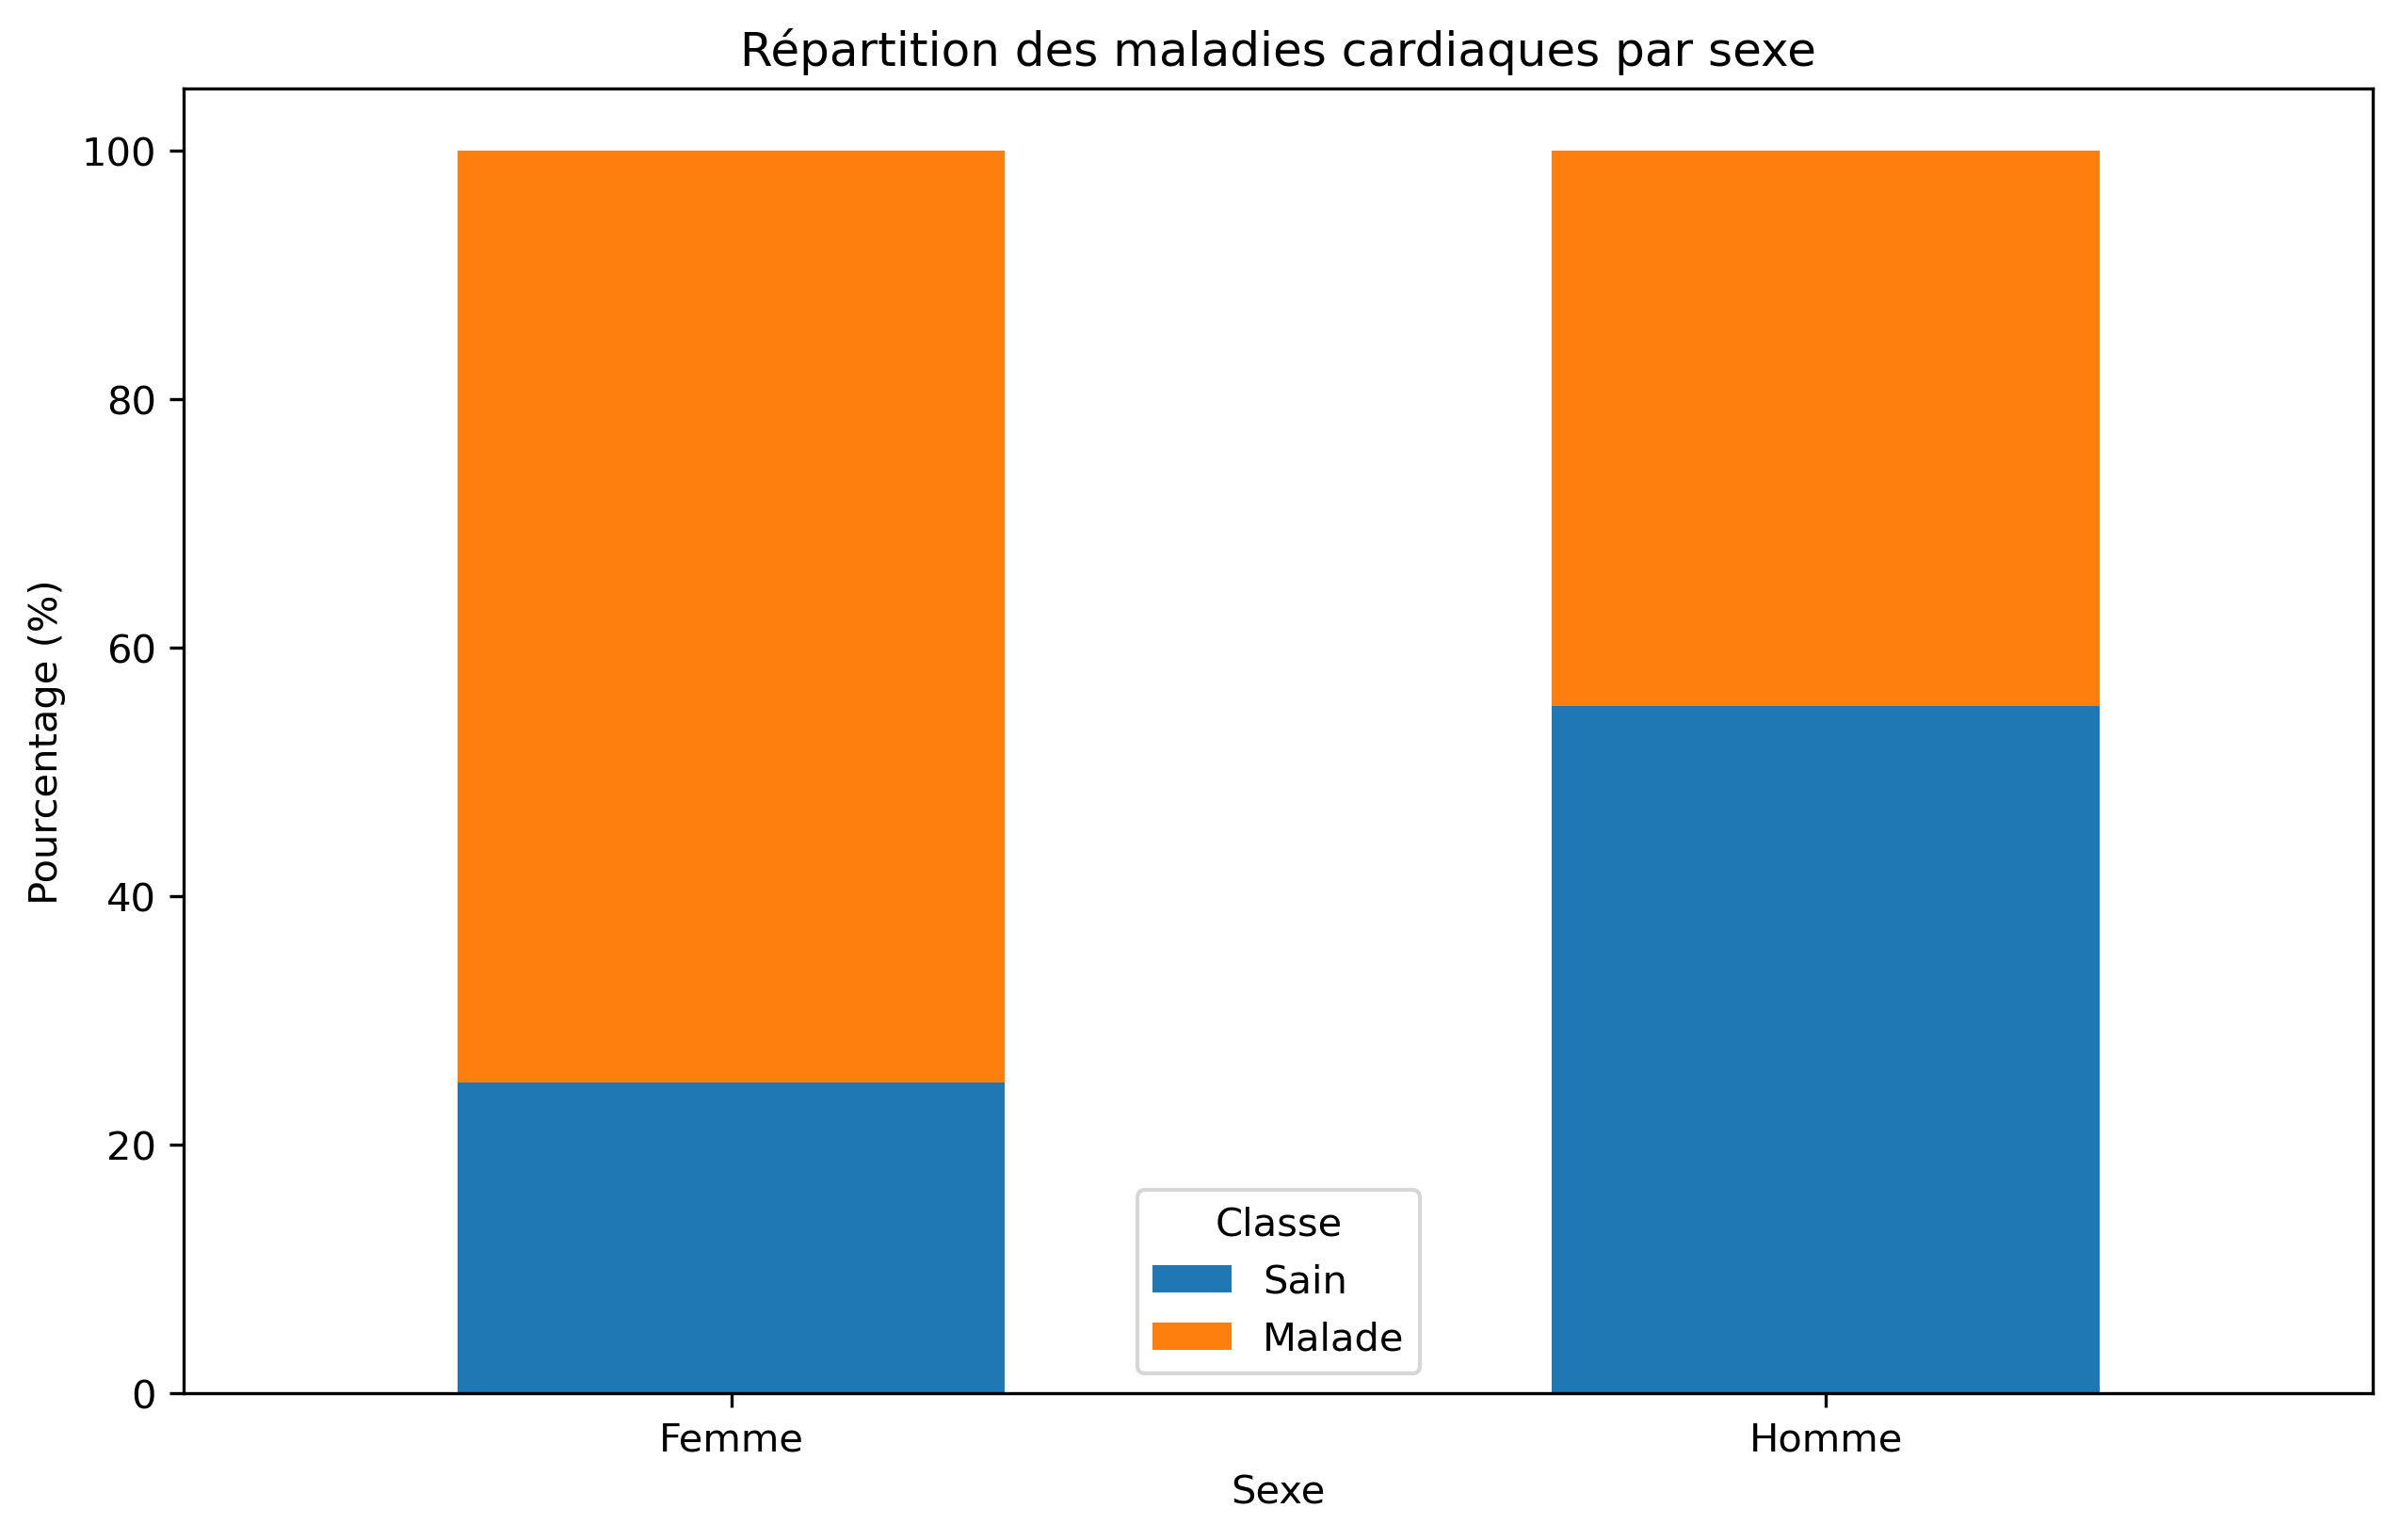
\includegraphics[width=1\textwidth]{./images/EDA/sex_rate_stacked.png}
			\caption{Distribution de la variable cible par sexe}
		\end{figure}

		% Modèles de machine learning
	\section{Modèles de Machine Learning et Entraînement}
		\subsection{Pipeline de préparation}

		Avant l'entraînement, les données sont séparées en un ensemble d'entraînement et un ensemble de test selon un ratio \textbf{80/20} avec stratification sur la variable cible.

		\begin{lstlisting}[style=pythonstyle, caption={Split stratifié 80/20}]
X = df.drop('target', axis=1)
y = df['target']

X_train, X_test, y_train, y_test = train_test_split(
	X, y, test_size=0.2, random_state=42, stratify=y)

scaler = StandardScaler()
X_train_sc = scaler.fit_transform(X_train)
X_test_sc  = scaler.transform(X_test)
		\end{lstlisting}
		\textbf{La Standardisation }(\texttt{StandardScaler})  est appliquée pour les modèles sensibles à l'échelle des features (Régression Logistique et KNN), mais pas pour la Forêt Aléatoire qui est invariante à l'échelle.
		\subsection{Modèles entraînés}

			\subsubsection{Régression Logistique (LR)}

				\begin{tcolorbox}[infobox, title={Régression Logistique}]
				\textbf{Paramètres :} solver = LBFGS · C = 1{,}0 · max\_iter = 1000 \\
				\textbf{Principe :} Modèle linéaire qui estime la probabilité $P(Y=1 | X)$ via la fonction sigmoïde :
				$$P(Y=1|X) = \frac{1}{1 + e^{-(\beta_0 + \beta_1 x_1 + \cdots + \beta_p x_p)}}$$
				\textbf{Avantages :} Interprétabilité, rapidité, baselines solide \\
				\textbf{Limites :} Suppose une frontière de décision linéaire
				\end{tcolorbox}
			
			\subsubsection{Forêt Aléatoire (RF)}

				\begin{tcolorbox}[infobox, title={Random Forest}]
				\textbf{Paramètres :} n\_estimators = 200 · max\_depth = 10 · critère = Gini \\
				\textbf{Principe :} Ensemble de 200 arbres de décision entraînés sur des sous-échantillons bootstrap. La prédiction finale est la classe majoritaire (vote). \\
				\textbf{Avantages :} Robustesse au bruit, capture des non-linéarités, fournit les importances de features \\
				\textbf{Limites :} Moins interprétable qu'un arbre unique, plus coûteux en mémoire
				\end{tcolorbox}
			\subsubsection{K-Plus Proches Voisins (KNN)}

				\begin{tcolorbox}[infobox, title={K-Nearest Neighbors}]
				\textbf{Paramètres :} K = 7 · distance = Euclidienne \\
				\textbf{Principe :} Classifie un point selon la majorité de ses K plus proches voisins dans l'espace des features standardisées. \\
				\textbf{Avantages :} Non-paramétrique, adaptatif \\
				\textbf{Limites :} Sensible au choix de K, coûteux à l'inférence sur grands datasets, sensible aux outliers
				\end{tcolorbox}
		\subsection{Validation croisée}

			Une \textbf{validation croisée stratifiée à 5 plis} (StratifiedKFold) est appliquée sur l'ensemble d'entraînement afin d'estimer la capacité de généralisation de chaque modèle et détecter un éventuel surapprentissage.

			$$\text{CV}_\mu = \frac{1}{5}\sum_{k=1}^{5} \text{Score}_k \qquad \text{CV}_\sigma = \sqrt{\frac{1}{5}\sum_{k=1}^{5}(\text{Score}_k - \text{CV}_\mu)^2}$$
	\section{Évaluation et Comparaison des Performances}

		\subsection{Métriques utilisées}

			Pour une tâche de classification binaire médicale, plusieurs métriques sont nécessaires :

			\begin{table}[H]
			\centering
			\caption{Définition des métriques d'évaluation}
			\label{tab:metrics}
			\begin{tabularx}{\textwidth}{lX}
				\toprule
				\textbf{Métrique} & \textbf{Formule et interprétation} \\
				\midrule
				Accuracy    & $\frac{TP+TN}{TP+TN+FP+FN}$ — proportion globale de bonnes prédictions \\[6pt]
				Précision   & $\frac{TP}{TP+FP}$ — parmi les cas prédits malades, combien le sont vraiment \\[6pt]
				Rappel      & $\frac{TP}{TP+FN}$ — parmi les vrais malades, combien sont correctement détectés \\[6pt]
				F1-Score    & $2 \cdot \frac{\text{Précision} \times \text{Rappel}}{\text{Précision} + \text{Rappel}}$ — compromis précision/rappel \\[6pt]
				AUC-ROC     & Aire sous la courbe ROC — capacité discriminante globale \\
				\bottomrule
			\end{tabularx}
			\end{table}

			\textbf{Note médicale :} Dans un contexte de dépistage cardiaque, le \textbf{rappel} (sensibilité) est particulièrement important : manquer un vrai malade (faux négatif) est plus grave que signaler un faux positif.
		\subsection{Résultats comparatifs}

			\begin{table}[H]
			\centering
			\caption{Tableau comparatif des performances sur l'ensemble de test}
			\label{tab:results}
			\begin{tabular}{lccccccc}
				\toprule
				\textbf{Modèle} & \textbf{Acc.} & \textbf{Prec.} & \textbf{Rappel} & \textbf{F1} & \textbf{AUC} & \textbf{CV Moy.} & \textbf{CV Std} \\
				\midrule
				Logistic Reg.   & 78{,}69\% & 76{,}32\% & 87{,}88\% & 81{,}69\% & 86{,}47\% & 81{,}34\% & $\pm$6{,}53\% \\
				Random Forest & 80{,}33\% & 75{,}61\% & 93{,}94\% & 83{,}78\% & 88{,}64\% & 83{,}41\% & $\pm$7{,}07\% \\
				KNN             & \best{81{,}97\%} & \best{78{,}95\%} & 90{,}91\% & \best{84{,}51\%} & \best{89{,}12\%} & 80{,}09\% & $\pm$2{,}73\% \\
				\bottomrule
			\end{tabular}
			\end{table}

			\begin{tcolorbox}[resultbox, title={Meilleur modèle : KNN $\bigstar$}]
			\begin{itemize}
				\item \textbf{F1-Score} : 84{,}51\,\% (meilleur compromis précision/rappel)
				\item \textbf{AUC-ROC} : 89{,}12\,\% (excellente capacité discriminante)
				\item \textbf{Accuracy} : 81{,}97\,\% sur l'ensemble de test
				\item \textbf{CV 5-fold} : 80{,}09\,\% $\pm$ 2{,}73\,\% (bonne généralisation)
			\end{itemize}
			\end{tcolorbox}		
\end{document}